%%% The main file. It contains definitions of basic parameters and includes all other parts.

%% Settings for single-side (simplex) printing
% Margins: left 40mm, right 25mm, top and bottom 25mm
% (but beware, LaTeX adds 1in implicitly)
\documentclass[12pt,a4paper]{report}
\setlength\textwidth{145mm}
\setlength\textheight{247mm}
\setlength\oddsidemargin{15mm}
\setlength\evensidemargin{15mm}
\setlength\topmargin{0mm}
\setlength\headsep{0mm}
\setlength\headheight{0mm}
\setlength{\columnseprule}{0.2pt}
% \openright makes the following text appear on a right-hand page
\let\openright=\clearpage

%% Settings for two-sided (duplex) printing
% \documentclass[12pt,a4paper,twoside,openright]{report}
% \setlength\textwidth{145mm}
% \setlength\textheight{247mm}
% \setlength\oddsidemargin{14.2mm}
% \setlength\evensidemargin{0mm}
% \setlength\topmargin{0mm}
% \setlength\headsep{0mm}
% \setlength\headheight{0mm}
% \let\openright=\cleardoublepage

%% Generate PDF/A-2u
\usepackage[a-2u]{pdfx}

%% Character encoding: usually latin2, cp1250 or utf8:
\usepackage[utf8]{inputenc}

%% Prefer Latin Modern fonts
\usepackage{lmodern}

%% Further useful packages (included in most LaTeX distributions)
\usepackage{amsmath}        % extensions for typesetting of math
\usepackage{amsfonts}       % math fonts
\usepackage{amsthm}         % theorems, definitions, etc.
\usepackage{bbding}         % various symbols (squares, asterisks, scissors, ...)
\usepackage{bm}             % boldface symbols (\bm)
\usepackage{graphicx}       % embedding of pictures
\usepackage{fancyvrb}       % improved verbatim environment
\usepackage{natbib}         % citation style AUTHOR (YEAR), or AUTHOR [NUMBER]
\usepackage[nottoc]{tocbibind} % makes sure that bibliography and the lists
			    % of figures/tables are included in the table
			    % of contents
\usepackage{dcolumn}        % improved alignment of table columns
\usepackage{booktabs}       % improved horizontal lines in tables
\usepackage{paralist}       % improved enumerate and itemize
\usepackage{xcolor}         % typesetting in color
\usepackage{paracol}
%%% Basic information on the thesis

% Thesis title in English (exactly as in the formal assignment)
\def\ThesisTitle{Artificial Intelligence for the Card Game Durak}

% Author of the thesis
\def\ThesisAuthor{Azamat Zarlykov}

% Year when the thesis is submitted
\def\YearSubmitted{2023}

% Name of the department or institute, where the work was officially assigned
% (according to the Organizational Structure of MFF UK in English,
% or a full name of a department outside MFF)
\def\Department{Department of Software and Computer Science Education (KSVI)}

% Is it a department (katedra), or an institute (ústav)?
\def\DeptType{Department}

% Thesis supervisor: name, surname and titles
\def\Supervisor{Adam Dingle, M.Sc.}

% Supervisor's department (again according to Organizational structure of MFF)
\def\SupervisorsDepartment{KSVI}

% Study programme and specialization
\def\StudyProgramme{Computer Science}
\def\StudyBranch{Artificial Intelligence}

% An optional dedication: you can thank whomever you wish (your supervisor,
% consultant, a person who lent the software, etc.)
\def\Dedication{%
I am filled with a sense of gratitude and admiration for my supervisor and professor Adam Dingle for his unwavering support and guidance throughout this process. His constant patience and dedication to helping in difficult moments have been a constant source of inspiration. His expertise and knowledge along with his willingness to go above and beyond to provide assistance have provided me with valuable insights, especially during the challenging times of writing my thesis. I am truly fortunate and lucky to have had the opportunity to learn from a such remarkable mentor. 

Moreover, I would like to thank my family and friends who have always been there for me during the process of writing my thesis. Their encouragement, advice, and participation in playing the Durak game to analyze the strategies have been invaluable to me and I am so grateful for a constant source of strength, and wisdom and for simply being there to provide a shoulder to lean on when I needed it the most.
}

% Abstract (recommended length around 80-200 words; this is not a copy of your thesis assignment!)
\def\Abstract{%
Because of its potential to improve the efficiency and effectiveness of many different fields, Artificial Intelligence (AI) has been the subject of extensive research and continues to be a major area of study. Given the numerous approaches to AI implementation, games provide a convenient and effective environment for testing and evaluating these algorithms. Nevertheless, card games with imperfect information present a unique challenge for many common game-playing algorithms because of their hidden game state. As a result, making them an active area of research in the field of game theory and AI. The objective of this thesis is to create a framework for implementing and testing various AI agents in the popular imperfect information card game "Durak" to identify the most effective approach in this environment. This paper presents a theoretical and experimental comparison of agents using various techniques, including rules-based heuristics, minimax search, and Monte Carlo tree search, to evaluate their effectiveness in the given context. In our analysis, we found that the Monte Carlo Tree Search agent performed the best among the implemented AI agents, whereas the rule-based heuristic agent and the minimax agent were less effective in the context of the imperfect information card game Durak.
}

% 3 to 5 keywords (recommended), each enclosed in curly braces
\def\Keywords{%
{artificial intelligence} {card game} {Durak}
}

%% The hyperref package for clickable links in PDF and also for storing
%% metadata to PDF (including the table of contents).
%% Most settings are pre-set by the pdfx package.
\hypersetup{unicode}
\hypersetup{breaklinks=true}

% Definitions of macros (see description inside)
%%% This file contains definitions of various useful macros and environments %%%
%%% Please add more macros here instead of cluttering other files with them. %%%

%%% Minor tweaks of style

% These macros employ a little dirty trick to convince LaTeX to typeset
% chapter headings sanely, without lots of empty space above them.
% Feel free to ignore.
\makeatletter
\def\@makechapterhead#1{
  {\parindent \z@ \raggedright \normalfont
   \Huge\bfseries \thechapter. #1
   \par\nobreak
   \vskip 20\p@
}}
\def\@makeschapterhead#1{
  {\parindent \z@ \raggedright \normalfont
   \Huge\bfseries #1
   \par\nobreak
   \vskip 20\p@
}}
\makeatother

% This macro defines a chapter, which is not numbered, but is included
% in the table of contents.
\def\chapwithtoc#1{
\chapter*{#1}
\addcontentsline{toc}{chapter}{#1}
}

% Draw black "slugs" whenever a line overflows, so that we can spot it easily.
\overfullrule=1mm

%%% Macros for definitions, theorems, claims, examples, ... (requires amsthm package)

\theoremstyle{plain}
\newtheorem{thm}{Theorem}
\newtheorem{lemma}[thm]{Lemma}
\newtheorem{claim}[thm]{Claim}

\theoremstyle{plain}
\newtheorem{defn}{Definition}

\theoremstyle{remark}
\newtheorem*{cor}{Corollary}
\newtheorem*{rem}{Remark}
\newtheorem*{example}{Example}

%%% An environment for proofs

\newenvironment{myproof}{
  \par\medskip\noindent
  \textit{Proof}.
}{
\newline
\rightline{$\qedsymbol$}
}

%%% An environment for typesetting of program code and input/output
%%% of programs. (Requires the fancyvrb package -- fancy verbatim.)

\DefineVerbatimEnvironment{code}{Verbatim}{fontsize=\small, frame=single}

%%% The field of all real and natural numbers
\newcommand{\R}{\mathbb{R}}
\newcommand{\N}{\mathbb{N}}

%%% Useful operators for statistics and probability
\DeclareMathOperator{\pr}{\textsf{P}}
\DeclareMathOperator{\E}{\textsf{E}\,}
\DeclareMathOperator{\var}{\textrm{var}}
\DeclareMathOperator{\sd}{\textrm{sd}}

%%% Graphics extensions 
\DeclareGraphicsExtensions{.png, .pdf}

%%% Transposition of a vector/matrix
\newcommand{\T}[1]{#1^\top}

%%% Various math goodies
\newcommand{\goto}{\rightarrow}
\newcommand{\gotop}{\stackrel{P}{\longrightarrow}}
\newcommand{\maon}[1]{o(n^{#1})}
\newcommand{\abs}[1]{\left|{#1}\right|}
\newcommand{\dint}{\int_0^\tau\!\!\int_0^\tau}
\newcommand{\isqr}[1]{\frac{1}{\sqrt{#1}}}

%%% Various table goodies
\newcommand{\pulrad}[1]{\raisebox{1.5ex}[0pt]{#1}}
\newcommand{\mc}[1]{\multicolumn{1}{c}{#1}}




% Title page and various mandatory informational pages
\begin{document}
%%% Title page of the thesis and other mandatory pages

%%% Title page of the thesis

\pagestyle{empty}
\hypersetup{pageanchor=false}
\begin{center}

\centerline{\mbox{
\includegraphics[width=166mm]{../img/logo-en.pdf}}}

\vspace{-8mm}
\vfill

{\bf\Large BACHELOR THESIS}

\vfill

{\LARGE\ThesisAuthor}

\vspace{15mm}

{\LARGE\bfseries\ThesisTitle}

\vfill

\Department

\vfill

{
\centerline{\vbox{\halign{\hbox to 0.45\hsize{\hfil #}&\hskip 0.5em\parbox[t]{0.45\hsize}{\raggedright #}\cr
Supervisor of the bachelor thesis:&\Supervisor \cr
\noalign{\vspace{2mm}}
Study programme:&\StudyProgramme \cr
\noalign{\vspace{2mm}}
Study branch:&\StudyBranch \cr
}}}}

\vfill

% Zde doplňte rok
Prague \YearSubmitted

\end{center}

\newpage

%%% Here should be a bound sheet included -- a signed copy of the "bachelor
%%% thesis assignment". This assignment is NOT a part of the electronic
%%% version of the thesis. DO NOT SCAN.

%%% A page with a solemn declaration to the bachelor thesis

\openright
\hypersetup{pageanchor=true}
\pagestyle{plain}
\pagenumbering{roman}
\vglue 0pt plus 1fill

\noindent
I declare that I carried out this bachelor thesis independently, and only with the cited
sources, literature and other professional sources. It has not been used to obtain another
or the same degree.

\medskip\noindent
I understand that my work relates to the rights and obligations under the Act No.~121/2000 Sb.,
the Copyright Act, as amended, in particular the fact that the Charles
University has the right to conclude a license agreement on the use of this
work as a school work pursuant to Section 60 subsection 1 of the Copyright~Act.

\vspace{10mm}

\hbox{\hbox to 0.5\hsize{%
In \hbox to 6em{\dotfill} date \hbox to 6em{\dotfill}
\hss}\hbox to 0.5\hsize{\dotfill\quad}}
\smallskip
\hbox{\hbox to 0.5\hsize{}\hbox to 0.5\hsize{\hfil Author's signature\hfil}}

\vspace{20mm}
\newpage

%%% Dedication

\openright

\noindent
\Dedication

\newpage

%%% Mandatory information page of the thesis

\openright

\vbox to 0.5\vsize{
\setlength\parindent{0mm}
\setlength\parskip{5mm}

Title:
\ThesisTitle

Author:
\ThesisAuthor

\DeptType:
\Department

Supervisor:
\Supervisor, \SupervisorsDepartment

Abstract:
\Abstract

Keywords:
\Keywords

\vss}

\newpage

\openright
\pagestyle{plain}
\pagenumbering{arabic}
\setcounter{page}{1}


%%% A page with automatically generated table of contents of the bachelor thesis

\tableofcontents

%%% Each chapter is kept in a separate file
\chapter*{Introduction}
\addcontentsline{toc}{chapter}{Introduction}

Artificial Intelligence (AI) is a fast-growing field of computer science that focuses on the creation of intelligent machines that can simulate human cognition. In recent years, AI technology has been applied in a wide range of fields, including healthcare, finance, and transportation, with the goal of improving efficiency, accuracy, and decision-making. To gain insights into the capabilities and limitations of AI algorithms and techniques, many researchers have turned to games as a testing platform to evaluate and compare different methods as they provide a convenient and controllable environment to achieve the aforementioned goals. 

In recent decades, computer games have also gained popularity, similar to the growth of AI as a field of study. Due to its utility, the game industry has become one of the many fields that have sought to use AI to their advantage. Being a subject of extensive research, perfect information in two-player games has been a common focus in game theory, which has allowed the development of algorithms for a greater understanding of games. However, in a manner similar to the real world, situations in which all relevant information is available are not always present. Given the inherent 
characteristics of their environment, the design of algorithms for imperfect information games is more challenging. Therefore, this thesis seeks to contribute to this field by developing algorithms for the game "Durak".

Durak is a strategic card game that originated in Russia \citep*{website:PAGAT_DURAK}. It is played with a deck of cards and typically involves two to six players. Unlike the other games, the aim of the Durak is not to find a winner, but to find a loser. Players take turns attacking and defending in a series of rounds. During an attack, the attacking player leads with one or more cards, and the defending player must attempt to beat them by playing a higher-ranked card. If the defending player is unable or unwilling to do so, they must pick up all the cards. The goal of the game is to get rid of all of one's cards, and the player left holding cards at the end is declared the fool. 

Given the intricate nature of the game, a key objective is to ensure its correct development with all relevant details. As the game will include various AI agents, it is essential for the game model to provide a suitable interface for the integration of AI agents. 

Another goal of this thesis is to implement a range of AI players for the given game model. One of the benefits of introducing the agents for this game is that it will provide an opportunity to examine potential challenges associated with implementing AI for games of this type, as well as verify the suitability and usability of the game's API for this purpose.

After implementing the AI agents, the aim is to compare their performance in mutual play, with the objective of identifying the most effective technique. The AI players must not only win against all other agents but must also make moves quickly, ideally at least several moves per second on average. This requirement reflects the need for AI players to be both effective and efficient in their decision-making. This comparison will provide valuable insights into the strengths and weaknesses of the various AI approaches and will help to guide future work in this area. 


\chapter{Game Description}
The objective of this thesis is to develop a simulation of the Durak game, which would serve as an experimental environment for artificial intelligence agents using various techniques. By implementing the full range of gameplay mechanics, our aim is to create a comprehensive simulation that could be used to evaluate the performance of previously mentioned agents.

There are many variations of the Durak game that are played around the world. However, this thesis focuses on the most well-known version of the game, which is called Podkidnoy Durak (also known as ``fool with throwing in'')\citep*{website:PAGAT_PODKIDNOY_DURAK}. In this chapter, we will provide a thorough description of this particular variation, providing an in-depth analysis of its rules and gameplay mechanics.

\section{Terminology}
In this section, any unfamiliar or potentially confusing terminology is defined to facilitate understanding of the material.

\begin{itemize}


        \item Trump card \\
        It is a playing card that belongs to a deck and has a higher rank than any other card from a different suit. This card is typically used strategically during gameplay to defeat the other player's cards and gain an advantage.
        \item Bout \\
         It is a process of exchange of attacks and defenses between the players. The bout continues until either the attack is successfully defended or the defender is unable to play a suitable card, at which point the attacker wins the bout and the defender is forced to take the played cards into their hand.
        \item Discard pile \\
         During a bout, if an attack is successfully defended, all of the cards played during this process are placed face down on a discard pile and are not used again for the remainder of the game.

\end{itemize}

\section{Players}
While the game of Durak is typically played with a range of two to six players, allowing for the possibility of team play, this work only focuses on the two-player variant of the game. This decision is made in order to maintain a consistent and focused scope for the analysis.

\section{Cards}
The game is played with a 36-card deck, which is divided into four suits: hearts, spades, clubs, and diamonds. The ranks of the cards within each suit are ranked from high to low as follows: ace, king, queen, jack, 10, 9, 8, 7, 6.

\section{Dealing the cards}
At the beginning of the game, cards are dealt to each player until each has a hand of six cards. The final card of the deck is then placed face up, and its suit is used to determine the trump suit for the game. The remaining undealt cards are then placed in a stack face down on top of the trump card.

During the first hand of a session, the player who holds the lowest trump card plays first. If no one holds the trump 6, the player with the trump 7 plays first; if no one holds that card, the player with the trump 8 plays first, and so on. The first play does not have to include the lowest trump card; the player who holds the lowest trump card can begin with any card they choose. If neither player has a trump card, the player who goes first is randomly determined.

\section{Beating the card} 
\label{BeatingRule}
Before discussing the gameplay, it is necessary to establish what it means for an attacking card to be successfully defended. A card that is not a trump can be beaten by playing a higher card of the same suit, or by any trump card. A trump card can only be beaten by playing a higher trump card. It is important to note that a non-trump attack can always be beaten by a trump card, even if the defender also holds cards in the suit of the attack card. There is no requirement for the defender to ``follow suit'' in this case.

\section{Game play}
The game consists of a series of bouts. During each bout, the attacker begins by placing a card from their hand, face up, on the table in front of the defender. The defender may then attempt to defeat this card by playing a card of their own, face up. Once the attacking card is defeated, the attacker has the option to continue the attack or to end it. If the attack continues, the defender must attempt to defend against this additional card. This process continues until the attacking player is unable or unwilling to attack. Alternatively, if the defender is unable or unwilling to beat the attacking card, they must pick up that card along with other played cards on the table.

\subsection{Conditions on the attack}
\label{attackconditions}
Every attacking card except for the first one must meet the following conditions in order to be played by the attacker.

\begin{itemize}
    \item Each new attacking card played during a bout must have the same rank as a card that has already been played during that bout, whether it was an attacking card or a card played by the defender.
    \item The number of attacking cards played must not exceed the number of cards in the defender's hand.
\end{itemize}
The first attacking card can be any card from the attacker's hand.

\subsection{Successful defense}
The defender successfully beats off the entire attack if either of the following conditions is met:
\begin{itemize}
    \item the defender has successfully beaten all of the attack cards and the attacking player is unable or unwilling to continue the attack.
    \item the defender has no cards left in hand while defending.
\end{itemize}

Upon successful defense of an attack, all cards played during the bout are placed in the \textbf{discard pile} face down and are no longer eligible for use in the remainder of the game. On top of that, the roles of the players change i.e. the defender becomes the attacker and the attacker becomes the defender for the next bout.

Furthermore, if the defender decides to take the cards, the attacker may play additional cards as long as doing so does not violate the conditions of the attack. In this case, the defender is required to also accept these supplementary cards.

\section{Illustrative Gameplay Scenario}

For the purpose of demonstrating the mechanics of the game, we will consider a scenario in which there are two players, A and B, and it is currently player A's turn. In this particular instance of the game, player A is holding the 6$\textcolor{red}{\heartsuit}$, 8$\textcolor{black}{\clubsuit}$, 8$\textcolor{red}{\diamondsuit}$ and A$\textcolor{black}{\clubsuit}$, while player B has the 8$\textcolor{red}{\heartsuit}$, A$\textcolor{red}{\heartsuit}$, 6$\textcolor{black}{\spadesuit}$ and K$\textcolor{black}{\clubsuit}$ in their hand. It should also be noted that $\textcolor{black}{\spadesuit}$ are the trump suit for this round. Player A initiates the attack with 6$\textcolor{red}{\heartsuit}$, which is the lowest value card in their hand. Player B has the option to respond to player A's attack by playing one of the 8$\textcolor{red}{\heartsuit}$, A$\textcolor{red}{\heartsuit}$, 6$\textcolor{black}{\spadesuit}$ from their hand, as these cards conform to the rules outlined in section \ref{BeatingRule}. Alternatively, player B can take the card. If player B chooses to defend player A's attack by playing the 8$\textcolor{red}{\heartsuit}$, the turn returns to player A. According to the conditions of the attack specified in section \ref{attackconditions}, player A has the option to either end the attack or continue the offensive play by playing either the 8$\textcolor{black}{\clubsuit}$ or 8$\textcolor{red}{\diamondsuit}$ from their hand. In case player A decides to finish the attack, all the cards in the bout move to the discard pile. On the other hand, if player A decides to continue the attack by playing one of their remaining cards, such as the 8$\textcolor{red}{\diamondsuit}$, the bout will continue and the turn will pass to player B. Of the three remaining cards in player B's hand, the only one that can be used to defend against player A's current attack is the 6$\textcolor{black}{\spadesuit}$, a trump card. Assume that because of strategic reasons, player B decides to take the cards. Then, all the cards in the bout move to player B's possession.

\section{Drawing from the deck}
Once the bout is over, all players who have fewer than six cards in their hand must, if possible, draw enough cards from the top of the deck to bring their hand size back up to six. The attacker of the previous bout replenishes their hand first, followed by the defender. If there are not enough cards remaining in the deck to replenish all players' hands, then the game continues with the remaining cards.

\section{Endgame and Objective}
Once the deck runs out of cards, there is no further replenishment and the goal is to get rid of all the cards in one's hand. The player who is left holding cards at the end is the loser, also known as the fool (durak). As it was mentioned before, this game is characterized by the absence of a winner, with only a loser remaining at the end. 

However, it is not always the case. It is possible for the game to end as a draw. In the event that both the attacking and defending player possess the same number of cards and all of the attacking player's cards are successfully defended, the game ends in a draw.
\chapter{Game Analysis}

As described in the chapter \ref{GameDescription}, Durak is a game that requires players to consider a range of factors in order to play effectively. Given its intricate nature, this chapter will analyze the game from the game-theoretic perspective in order to understand its underlying structure and strategic considerations. This will involve categorizing the game according to relevant criteria, examining the complexity of the game as a whole, comparing the length of the game, introducing new concept and etc.

\section{The Termination of Durak}
It is essential to acknowledge that every game of Durak must eventually conclude, as it is not possible for a game to continue indefinitely. For a game to persist, players would need to repeatedly exchange the same set of cards. However, this scenario is not feasible because cards cannot return to a previous owner until certain cards from the bout are placed in the discard pile. The inclusion of cards in the discard pile allows for the changing of turns, enabling the return of previously exchanged cards to their original owner. As the exchange of cards between players continues, additional cards from the deck and ultimately from the players' hands will be placed in the discard pile until only the cards being exchanged remain.

\section{Repetition of States in Durak}
Another question of interest is whether it is possible for the same game state to occur twice within a single game of Durak. Despite the numerous exchanges of cards between players, it is not possible for the same game state to be replicated. For the same state to repeat, players would need to exchange the same set of cards in a circle, such as player A attacking with an Ace card and player B taking it, then player B attacking with the same Ace on the next turn to player A. However, this scenario is not feasible. As previously mentioned, the intermediate bout must come to an end and cards from it must be placed in the discard pile in order to allow player B to return the Ace to player A. By this point, the game state will have changed due to the presence of additional cards in the discard pile that were not present when the Ace belonged to player A. As a result, it is not possible for the same game state to repeat in a single game of Durak.

\section{The Advantage of the First Moving Player}
It is a common misconception that the first player to move in a game of Durak holds a significant advantage over their opponent. While it is true that the first player has the opportunity to set the tone of the game and establish their strategy from the outset, this advantage is not necessarily decisive. A skilled opponent can effectively counter the strategies of the first player and ultimately achieve victory. The outcome of a game of Durak is determined by the players' abilities and strategies, rather than the order in which they move.

\section{Classification}

Durak can be classified as a \textbf{discrete game}. A discrete game is a type of game in which players have a finite number of choices, or actions, that they can take \citep{Gametheory4}. This applies in Durak. Players have a limited number of choices that they can make at each turn. They can choose which card to play, and must decide whether to attack or defend. These choices are limited by the cards that the player has in their hand and the rules of the game. 

Furthermore, it can be considered a \textbf{sequential} game from a game-theoretic perspective. A sequential game is a type of game in which the order in which players make their decisions matters \citep{Gametheory4}. In Durak, the order in which players play their cards is important, as it determines who is able to attack and who must defend. The sequence of actions is determined by the rules of the game described in chapter \ref{GameDescription}, and players must consider the potential actions of their opponents as they make their own decisions. 

In addition, Durak can be classified as a game of \textbf{imperfect information}. In a game of imperfect information, players do not have complete information about the game state or the actions of their opponents \citep{Gametheory4}. They must make decisions based on incomplete information and must try to infer the actions of their opponents based on their observations and past experiences. As described before, Durak is a game of imperfect information because players do not have complete information about the cards in the hands of their opponents. They must make decisions about which cards to play and when to use their trump cards based on incomplete information, and must adapt their strategies as the game progresses and new information becomes available.

Additionally, Durak is often played in a \textbf{deterministic} manner, meaning that the outcome of the game is determined by the initial cards that are dealt and the actions that are taken by the players during the game. However, there is some element of chance in Durak, as the cards are shuffled randomly before the game begins can affect the outcome of the game. Therefore, it is possible to consider Durak to be a \textbf{non-deterministic} game to some degree. In game theory, a non-deterministic game is a type of game in which the outcomes are not determined solely by the actions of the players and the rules of the game, but are also influenced by random events or factors \citep{Gametheory4}. 

In summary, Durak can be classified as a discrete, sequential, imperfect information, and non-deterministic to some extent game from a game-theoretic perspective, which contribute to its complexity and strategic depth.


\section{Branching Factor}

The branching factor of a game refers to the number of possible moves that a player can make at each turn. In ``Podkidnoy Durak'', it can be challenging to determine the branching factor as it varies depending on the specific game state. At each turn, the number of possible moves a player can make is influenced by the cards in their hand and the cards on the table, as well as the defending or attacking rules. To be specific, the attacker can initiate an attack by playing any card from their hand. Therefore, the maximum branching factor is the maximum number of cards that a player can hold in their hand, which is 35 if one player holds all but one of the cards. However, there are also situations in which a player may only have one possible move, such as when they are unable to defend against an attack and must pass and take the card. Therefore, the average branching factor in this game is relatively low, as players often have only a few choices of cards to play in a given situation. This is particularly true for the defender, who may only have a few options for defending against an attack, and for subsequent attacks, where the number of available options may also be limited.

To clarify the branching factor assumption, I have run an experiment to estimate the average branching factor in Durak by simulating 1000 random games played between two greedy agents. The results showed that the average branching factor, as computed using the \textbf{geometric mean}, was \textbf{2.17}, which suggests that the branching factor of the game is low. 

\section{Duration}

The objective of this section is to determine the typical duration of games of Durak in terms of bouts and plies, where ply refers to a single move made by a single player. To address this question, we will compare the average length of games played between two random players and two greedy agents, in order to examine the influence of player strategy on the duration of the game.

To compare the durations of player strategies in Durak, we conducted two experiments. The first experiment involved 1000 games played between two greedy agents, and the second experiment involved 1000 games played between two random agents. The results of the first experiment showed that the average number of bouts per game was 8.3, the average number of plies per bout was 5.3, and the average number of plies per game was 44.0. The results of the second experiment showed that the average number of bouts per game was 24.0, the average number of plies per bout was 2.9, and the average number of plies per game was 68.0. These findings suggest that the behavior of the random agents led to longer games, as evidenced by the higher number of bouts and lower number of plies per bout in the second experiment.

\section{Weakness Concept}
\label{weaknessConcept}
This section introduces the concept of \textbf{weakness} and \textbf{well-covered weakness} in Durak, which are the concepts that arise from the analysis of the game and may be relevant to various strategies or agents.

The concepts in question are introduced in Edouard Bonnet's paper ``The Complexity of Playing Durak''. It examines the difficulty of identifying winning strategies in the card game Durak. Bonnet's work demonstrates that, even in a perfect information setting with two players, finding optimal moves is a challenging computational problem. Specifically, Bonnet establishes that determining the presence of a winning strategy in a generalized Durak position is PSPACE-complete. In my own research, I aim to construct a strong agent capable of playing optimally in both perfect and imperfect information settings. Bonnet's contributions, including the concept of weakness and well-covered weakness, have been invaluable in the development of my rule-based agents.

A weakness for a player, referred to as player \textit{P}, is defined as a rank \textit{r} that meets the following criteria: 
\begin{enumerate}
	\item player \textit{P}'s hand contains at least one card of rank \textit{r}, and
	\item for each suit \textit{s} of rank \textit{r} in player \textit{P}'s hand, there exists a rank $\textit{r}$'$ > \textit{r}$ such that the opponent holds a card of rank \textit{r}$'$ and suit \textit{s} \citep{Bonnet2016TheCO}.
\end{enumerate}

To clarify the concept of weakness, consider the following scenario: Player P holds the cards 10$\textcolor{red}{\heartsuit}$, 10$\textcolor{black}{\spadesuit}$, and K$\textcolor{red}{\diamondsuit}$, while player O holds Q$\textcolor{red}{\heartsuit}$, Q$\textcolor{black}{\spadesuit}$, and J$\textcolor{black}{\clubsuit}$. In this case, player P has a weakness at rank 10, as it satisfies the two conditions outlined in the definition of weakness. Specifically, player P holds at least one card of rank 10 (10$\textcolor{red}{\heartsuit}$ and 10$\textcolor{black}{\spadesuit}$), and for each suit of rank 10 in player P's hand (10$\textcolor{red}{\heartsuit}$ and 10$\textcolor{black}{\spadesuit}$), the opponent holds a card of higher rank (Q$\textcolor{red}{\heartsuit}$ and Q$\textcolor{black}{\spadesuit}$, respectively).

A well-covered weakness for player \textit{P}, on the other hand, refers to a weakness card with rank \textit{r} such that for every card in player \textit{P}'s hand with suit \textit{s} and rank \textit{r}, there is a higher card with suit \textit{s} and rank \textit{r}' in player \textit{O}'s hand, and player \textit{P} does not possess any cards with rank \textit{r}'. Essentially, if player \textit{P} attacks with a well-covered weakness, player \textit{O} can defend effectively, preventing player \textit{P} from playing any other attacking cards during the bout.

In the example provided following the definition of weakness, the cards 10$\textcolor{red}{\heartsuit}$ and 10$\textcolor{black}{\spadesuit}$ are considered well-covered weaknesses because attacking with these cards allows the opponent, player O, to effectively defend with Q$\textcolor{red}{\heartsuit}$ and Q$\textcolor{black}{\spadesuit}$ and prevent player P from attacking again.

\section{Closed World Deduction}

In the closed world environment, it is possible for a player to deduce the opponent's remaining cards once the deck is depleted. This is because once the deck is exhausted, the only cards that can be played are those that are held by the players. If a player is able to keep track of the cards that have been played, they can narrow down the possible cards that their opponent still holds and make educated guesses about their strategy based on this information. To give an example, imagine that the deck has been exhausted, and there are only four cards left in the game: A$\textcolor{red}{\heartsuit}$, 6$\textcolor{black}{\spadesuit}$, 7$\textcolor{red}{\diamondsuit}$, and 8$\textcolor{black}{\clubsuit}$. Player A is able to deduce that their opponent, player B, still holds A$\textcolor{red}{\heartsuit}$ because they have played the 6, 7, and 8 cards, but have not yet played the A card. Based on this information, player A can infer that player B is likely trying to hold onto the A card in order to use it as a trump card later in the game. By paying a close attention, player A will know which cards have already been played and which ones are still in play. Player A knows that A$\textcolor{red}{\heartsuit}$ has not yet been played because they have not seen it played, and they also know that the A$\textcolor{red}{\heartsuit}$ card has not been discarded because the deck has not yet been exhausted. Therefore, player A can deduce that the A$\textcolor{red}{\heartsuit}$ card is still in play either in the deck or in the opponent's hand. Once the deck is depleted, it becomes obvious that it is being held by player B. The ability to deduce an opponent's remaining cards can significantly impact the course of the game, as it allows players to incorporate this information into their strategic decision-making. However, it is important to note that Durak is a game of chance as well as strategy, and even if a player is able to deduce their opponent's remaining cards, they cannot predict with certainty which cards the opponent will play in a given turn. 
\chapter{Game and AI Implementation}

The primary objective of this study is to design and develop a framework for the implementation and evaluation of artificial intelligence (AI) agents in Durak. Since the framework in this game is tailored to support the application and evaluation of AI algorithms within the game environment, the focus of this chapter is to provide a high-level overview of the framework's architecture, including its capabilities for supporting the development and evaluation of AI agents for Durak.

\section{OS support}

I tested the game framework for Durak on both the Windows 10 and Linux operating systems to confirm compatibility and functionality. While this list is not exhaustive, and the framework may potentially run on other operating systems, these are the only ones that were formally tested.

\section{A High-Level View of the Framework}

The Durak AI framework includes a game model, AI agents, and a command-line interface (CLI) that are implemented using the C\# programming language and targeted for the .NET 6 platform.

In order to run and test the program, the project has to be cloned from the repository . The source code for the project is available on the project GitHub page \citep{DurakRepo}. From the CLI directory of the project, the user can use the command line to enter the following command: 
\begin{lstlisting}
$ dotnet run
\end{lstlisting}
This will launch the command-line interface and provide guidance on how to proceed with experimentation (for additional information, please refer to Section \ref{CLI}).

An analysis of the source code using Visual Studio's Calculate Code Metrics for Solution feature revealed that the solution consists of a total of 3034 lines of source code. This includes 993 lines in the Agent project, 757 lines in the CLI project, and 1284 lines in the game model.

\subsection{Project Structure}
The game Durak is organized within a solution file, with the file extension ``.sln'', which is a type of file used to manage projects in Visual Studio. This solution includes three individual projects: 

\begin{itemize}

\item \textbf{Model} - A C\# library project that contains the game logic for Durak.

\item \textbf{Agent} - A C\# library that contains all of the implemented AI agents.

\item \textbf{CLI} - A C\# Command-Line Interface (CLI) project that includes parameters for modifying the game model and agents settings in order to perform experiments.

The aforementioned components will be further discussed in the following subsections.

\end{itemize}

\subsection{Model}

The game model, which represents the current state of the game, is implemented using object-oriented programming principles. As was mentioned before, the game logic for Durak is contained within the \textbf{Model} C\# library, which serves as a modular and reusable unit. It includes class objects, such as \texttt{Player}, \texttt{Card}, and \texttt{Deck}, as well as all of the other main components that make up the game. 

\begin{figure}[h]
    \centering
    \captionsetup{justification=centering}
    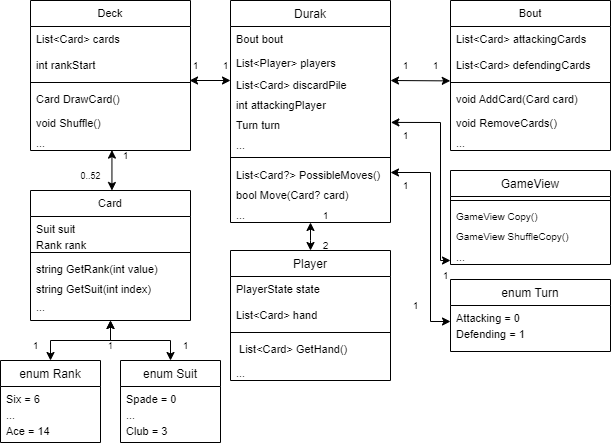
\includegraphics[width=0.9\textwidth]{../img/modelUML.png}
    \caption{A simplified UML diagram showing the relationship between the objects within the Model library.}
    \label{fig:modelUML}
\end{figure}

Before delving into the description of the game state and components of Durak, it is useful to first consider the relationship of all of the objects in the model to that state. A class diagram illustrating the relationships between the objects in the model can be found in Figure \ref{fig:modelUML}.

The \texttt{Deck} object includes the property \texttt{rankStart}, which is an integer value that can be modified from the command-line to alter the starting rank of the cards in the deck. By default, the \texttt{rankStart} is set to 6, but it can be changed to any value between 6 and 14. For instance, if the \texttt{rankStart} is set to 13, the deck will only consist of 8 cards: 4 Aces (rank value 14) and 4 Kings (rank value 13). 

The representation of the game state \texttt{Durak} in the model is a key aspect of the overall system. This representation holds all of the necessary information and logic required to play the game of Durak, shown in Figure \ref{fig:codeDurak}, and therefore plays a central role in the functioning of the model. As such, it is important to carefully consider the design and implementation of the game state representation along with its components. 

\begin{figure}[h]
\captionsetup{justification=centering}
\begin{lstlisting}
// Bout object of the game
private Bout bout;

// Deck object of the game
private Deck deck;

// Trump card of the game that can be assigned or not
private Card? trumpCard;

// Representation of the discard pile in the game
private List<Card> discardPile = new List<Card>();

// Players inside the game
private List<Player> players = new List<Player>();

\end{lstlisting}
\caption{A simplified diagram of the Durak class, which encompasses the main properties of the game}
\label{fig:codeDurak}
\end{figure}

The object in question serves as a comprehensive representation of all game states and data throughout a single game of Durak. To facilitate communication and coordination between the Durak model and the agents that interact with it, the game state provides two primary functions: \texttt{PossibleMoves}, shown in Figure \ref{fig:codePossibleMoves} and \texttt{Move}, shown in Figure \ref{fig:codeMove}. These functions serve as the primary means of interaction between agents and the game state, and as such, play a crucial role in the overall operation of the model. 

\begin{figure}[h]
\captionsetup{justification=centering}
\begin{lstlisting}
if (turn == Turn.Attacking){
    if (CanAttack() && OpponentCanFitMoreCards()) {
        return GenerateListOfAttackingCards();
    } else {
        // passing the attack
        return null;	
    }
}
else {
    Card attackingCard = bout.GetAttackingCards()[^1]
    if (CanDefend(attackingCard)) {
        return GenerateListofDefendingCards(attackingCard);
    } else {
        // taking the cards
        return null
    }
}
\end{lstlisting}
\caption{A simplified overview of the PossibleMoves method inside the Durak class}
\label{fig:codePossibleMoves}
\end{figure}

The \texttt{PossibleMoves} method determines the list of actions that are available to the current player based on the current game state and the rules of the game. When it is the attacker's turn, the method considers the rules for attacking (details in section \ref{attackconditions}) and generates a list of eligible cards that can be played or allows the player to pass if no suitable cards are available. Similarly, when it is the defender's turn (details in section \ref{BeatingRule}), the method takes into account the card being attacked and generates a list of cards that can be played to defend or offers the option to take the attack if no suitable defense is available. Because of that the \texttt{PossibleMove} function returns \texttt{List<Card?>} type. If there are possible moves that can be made in the current state, the function returns a list of the available cards to play. If no moves can be made, the function returns a list containing a single \texttt{null} element, which indicates that the current player must pass or take the card or cards from the bout, depending on the current turn. It should be noted that the example provided in Figure \ref{fig:codePossibleMoves} is a simplified version that omits certain implementation details, such as the process of adding elements to the list. 

\begin{figure}[h]
\captionsetup{justification=centering}
\begin{lstlisting}
if (!ValidAction(card, attacker, defender)) 
    return false;
	
if (turn == Turn.Attacking){
    if (card is not null) {
        attacker.GetHand().Remove(card);
        bout.AddCard(card);
    } else {
        bout.RemoveCards();
        return true;
    }
}
else {
    if (card is not null){
        defender.GetHand().Remove(card);
        bout.AddCard(card);
    } else {
        FillPlayerHand(bout.GetEverything(), defender)
        return true;
    }	
}
turn = turn == Turn.Attacking ? Turn.Defending : Turn.Attacking;
return true;
\end{lstlisting}
\caption{A simplified overview of the Move method inside the Durak class}
\label{fig:codeMove}
\end{figure}

The \texttt{Move} method modifies the current game state by executing the action chosen by the current player. This move is selected by the agent, which performs calculations based on the possible moves generated by the \texttt{PossibleMoves} method. The specific nature of these calculations depends on the type of agent being used. For example, a rule-based agent may simply select the lowest value rank card, while a more sophisticated agent, such Monte-Carlo Tree Search (MCTS), may use more complex decision-making processes to determine the optimal move to make. Regardless of the type of agent being used, the \texttt{Move} method ultimately updates the game state to reflect the chosen action and advances the game to the next turn. To implement the desired changes, the \texttt{Move} method accepts a parameter of type \texttt{Card?}. This parameter represents the move made by the agent, which can be a card play (type \texttt{Card}), or a pass or draw (type \texttt{null}), depending on the role of the agent. Also, it is worth noting that the \texttt{Move} method returns a boolean value. In order to prevent invalid moves, the method verifies the validity of the intended action before making any changes. If the action is deemed valid, the method returns true; otherwise, it returns false.

Additionally, it is important to note that, for efficiency and security purposes, the agents are not provided with the entire \texttt{Durak} object. One reason is that the Durak class contains a large amount of data and methods that are not relevant to the agents' decision-making process. By providing a smaller class such as \texttt{GameView} that only includes the necessary information, such as methods outlined in Figures \ref{fig:codePossibleMoves} and \ref{fig:codeMove}, the agents can more efficiently access the information they need and ignore the rest. Another reason is that the Durak class contains sensitive or proprietary information that should not be shared with the agents. By using a smaller class such as \texttt{GameView} to provide the necessary information, it is possible to control what information is exposed to the agents and protect any sensitive data.

Other than \texttt{PossibleMoves} and \texttt{Move} methods, the \texttt{Copy} method is an important feature of the \texttt{GameView} object worth mentioning. This method creates a duplicate of the current game state, which is useful for game tree exploration by agents such as Minimax and MCTS, due to their need to examine multiple potential moves and outcomes. For further information on the use of the \texttt{Copy} method in Minimax and MCTS, please refer to section \ref{minimax} and \ref{MCTS} of the text.

\subsection{CLI}
\label{CLI}

The command-line interface (CLI) plays a crucial role in the architecture of the application. Through the CLI, the user can interact with the application using a text-based interface, providing parameters and receiving feedback or results. The CLI enables a range of experimental and testing scenarios, including the ability to conduct playouts between different agents within a customizable game environment that can be modified by altering various parameters. In this section, we will examine the various parameters that can be used to manipulate the behavior of the agents and the game environment through the CLI.

Before discussing the organizational structure of the project, it is important to introduce the parameters and their roles within the project (please refer to Table \ref{paramsTable}).

\begin{table}
\captionsetup{justification=centering}
\begin{center}
\resizebox{\textwidth}{!}{%
\begin{tabular}{ | m{0.2\textwidth} | m{0.8\textwidth}| } 
  \hline
   Parameter & Description \\
  \hline
  -ai1 & The agent for player 1. (String) (Default = random) \\ 
  \hline
  -ai2 & The agent for player 2. (String) (Default = random) \\ 
  \hline
  -d1 & Displays \# of states \& depth for minimax move (Default = False) \\ 
  \hline
  -d2 & Displays all the moves that minimax considers (Default = False) \\ 
  \hline
  -include\_trumps & Enable trump cards in the game (Default = True) \\ 
  \hline
  -log & Enable logs for writing in the file (Default = False) \\ 
  \hline
  -open\_world & Make all cards visible to both players (Default = False) \\ 
  \hline
  -seed & A seed for random number generation (Int32) \\ 
  \hline
  -start\_rank & The starting rank of cards in the deck (Int32)(Default = 6) \\ 
  \hline
  -total\_games & The number of games to play (Int32)(Default = 1000) \\ 
  \hline
  -tournament & Runs the tournament with the agents specified. \\ 
  \hline
  -verbose & Enable verbose output (Default = False) \\
  \hline
\end{tabular}}
\end{center}
\caption{\label{paramsTable} Command-line parameters}
\end{table}

The \texttt{-open\_world} parameter plays a key role in determining the level of information available to players in the game. If the \texttt{-open\_world} parameter is present, the game environment is fully visible to all players, including the cards in the deck and the cards in players' hands. This results in a perfect information environment, where all players have access to the same information. By comparing agents in this type of environment, it is possible to identify the most effective one. On the other hand, if the \texttt{-open\_world} parameter is not present, the game environment is not fully visible to all players, resulting in an imperfect information environment where players may not have complete knowledge of the game state

The \texttt{-tournament} parameter allows for the specified agents to engage in a series of games, the results of which are recorded in a CSV file. The game settings for the tournament can be customized when the \texttt{-tournament} parameter is included. These settings will be applied to all games played between the agents. However, if the results of the games between two agents do not show a significant difference according to Wilson's score, the number of games will be increased by 500 and the tournament will be restarted for two equally strong agents in order to ensure that the best player can be accurately determined. There is an upper limit on the number of games that can be played in cases where the agents are evenly matched and unable to produce a clear winner. In such situations, the agents will be listed in a separate table within the CSV file. An example of how to initiate a tournament between the Random, Greedy, and Smart agents is provided below:

\begin{lstlisting}
$ dotnet run -tournament="random/greedy/smart" -total_games=100
\end{lstlisting}

There are various ways to utilize the parameters in Table \ref{paramsTable}. An example of using the default settings to run a game between RandomAI agent(\texttt{random}) and GreedyAI agent(\texttt{greedy}) is provided below.

\begin{lstlisting}
$ dotnet run -ai1=random -ai2=greedy
\end{lstlisting}

This command initiates the simulation of 1000 games between the RandomAI and GreedyAI agents in a fully enclosed environment, where players can only see their own cards and not those of other players, (with a starting rank of 6) and provides the following output to the console:

\begin{lstlisting}
==== RUNNING ====

Game 1: Agent 1 (random) won. Total bouts: 21
Game 2: Agent 2 (greedy) won. Total bouts: 19
Game 3: Agent 2 (greedy) won. Total bouts: 13
Game 4: Agent 2 (greedy) won. Total bouts: 18
Game 5: Agent 2 (greedy) won. Total bouts: 18
...
\end{lstlisting}

To more thoroughly analyze the results of any specific game, \texttt{seed} with the game id and the \texttt{-verbose}  parameters may be utilized. This provides detailed information about the progression of the game by showing every possible move, the chosen move and other game related details. An example of the first game in which a RandomAI agent defeats a GreedyAI agent using this parameter is shown below:


\begin{lstlisting}
$ dotnet run -ai1=random -ai2=greedy -verbose -seed=1
\end{lstlisting}

The command above generates verbose output, as shown below. It should be noted that this is only a portion of the full output and the blue colored suits are the indications of the trump suit.

\begin{lstlisting}
==== START ====

Trump card: A(*@$\textcolor{blue}{\diamondsuit}$@*)
Deck's size: 36

Player 1 (random) cards: 9(*@$\textcolor{black}{\spadesuit}$@*)  A(*@$\textcolor{black}{\spadesuit}$ @*) 10(*@$\textcolor{red}{\heartsuit}$@*)  Q(*@$\textcolor{red}{\heartsuit}$@*)  9(*@$\textcolor{blue}{\diamondsuit}$@*)  K(*@$\textcolor{blue}{\diamondsuit}$@*)
Player 2 (greedy) cards: 6(*@$\textcolor{black}{\spadesuit}$@*)  8(*@$\textcolor{black}{\spadesuit}$@*)  Q(*@$\textcolor{black}{\spadesuit}$@*)  7(*@$\textcolor{red}{\heartsuit}$@*)  A(*@$\textcolor{red}{\heartsuit}$@*)  6(*@$\textcolor{black}{\clubsuit}$@*)

=== New Bout ===

TURN: Player 1 (random) (Attacking)
Can attack
Possible cards: 9(*@$\textcolor{black}{\spadesuit}$@*)  A(*@$\textcolor{black}{\spadesuit}$@*)  10(*@$\textcolor{red}{\heartsuit}$@*)  Q(*@$\textcolor{red}{\heartsuit}$@*)  9(*@$\textcolor{blue}{\diamondsuit}$@*)  K(*@$\textcolor{blue}{\diamondsuit}$@*)
Attacks: 9(*@$\textcolor{black}{\spadesuit}$@*)

Bout 1:
Attacking cards: 9(*@$\textcolor{black}{\spadesuit}$@*)
Defending cards:

TURN: Player 2 (greedy) (Defending)
Can defend
Possible cards: Q(*@$\textcolor{black}{\spadesuit}$@*)
Defends: Q(*@$\textcolor{black}{\spadesuit}$@*)

Bout 1:
Attacking cards: 9(*@$\textcolor{black}{\spadesuit}$@*)
Defending cards: Q(*@$\textcolor{black}{\spadesuit}$@*)
...
\end{lstlisting}

\textbf{Reproducibility} is a critical aspect of scientific experimentation. In this context, reproducibility refers to the ability to obtain the same results by running the program with the same command line parameters. To ensure reproducibility, the program assigns a unique identifier to each game, which serves as a seed for the random number generator that deals cards to players. This allows testing  different agents in a controlled and consistent environment, facilitating comparison of performance and error detection.

Upon completion of an experiment, the program presents statistical analysis on all simulations conducted using the specified game and agent configuration. This analysis includes various metrics, such as the average number of bouts played per game, the average number of plies made per bout, the average time taken per ply by each agent, the win rate, and the \textbf{Wilson confidence interval} between the two agents.

\begin{figure}[h]
\captionsetup{justification=centering}
\begin{lstlisting}
$ dotnet run -ai1=greedy -ai2=random -open_world -total_games=1000 
			-start_rank=6 -include trumps
...

==== STATISTICS ====
Total games played: 1000

Average bouts played over the game: 17.1
Average plies per bout over the game: 3.1
Average plies played over the game: 52.0
Average time per move (greedy agent): 0.0060ms
Average time per move (random agent): 0.0058ms

Draw rate: 0.8%
Agent 1 (greedy) won 913 / 1000 games (91.3%)
Agent 2 (random) won 79 / 1000 games (7.9%)

With 98% confidence, Agent 1 (greedy) wins between 89.8% and 93.8%
With 98% confidence, Agent 2 (random) wins between 6.2% and 10.2%
\end{lstlisting}
\caption{A representation of command and statistics.}
\label{fig:statistics}
\end{figure}

I chose Wilson's confidence interval in order to assess the statistical significance of the observed difference in win rates between the two players. By using this measure, we may determine whether the observed difference in win rates was likely to be a true reflection of the relative abilities of the players, or whether it may have occurred by chance \citep{moore_mccabe_craig_2017}. Overall, the statistical data generated from the simulations was useful for identifying potential errors and for optimizing the strategies for the rule-based agents. As an example, Figure \ref{fig:statistics}  presents the statistical result of a simulation comparing the performance of greedy and random agents in a full open-world game.

Other than that, it is important to consider that when utilizing certain advanced agents, such as Monte-Carlo Tree Search (MCTS) and Minimax, it is necessary to specify their respective parameters in order to effectively utilize their capabilities. Those parameters will be discussed in Section \ref{paramSpecification}.

\subsection{Agent}

The Agent library is a collection of artificial intelligence agents that are utilized in the experiment. The agents included in this library are: Random, Greedy, Smart, Minimax, and MCTS. The functionality and implementation of these agents will be elaborated upon in the next chapter. This section describes the overall structure and organization of the Agent library.

The abstract class \texttt{Agent} represents a common interface for all agents. The program calls the \texttt{Move} method to ask an agent which move it will make in a given game state. A visual representation of the abstract class \texttt{Agent} is provided in Figure \ref{fig:abstractClass}.

\begin{figure}[h]
\captionsetup{justification=centering}
\begin{lstlisting}
public abstract class Agent
{
    public string? name;
    public string? GetName() => name;
    public abstract Card? Move(GameView gameView);
}
\end{lstlisting}
\caption{A representation of the abstract class 'Agent'}
\label{fig:abstractClass}
\end{figure}

As an example, we can examine the behavior of a Random agent, which selects a move from the list of possible moves at random, can be examined. This process is demonstrated in Figure \ref{fig:randomMove}. The \texttt{Move} method of the Random agent is responsible for implementing this behavior. The figure illustrates the process of overriding the abstract \texttt{Move} method in order to modify the behavior of the function based on the random nature. This process is followed for all agents that must implement this method, resulting in diverse behaviors depending on the agent in question.
\chapter{Artificial Intelligence Agents}
\label{AIAgents}

Durak features five distinct artificial intelligence (AI) agents: Random, Greedy, Smart, Minimax, and MCTS. In this chapter, we will delve into the characteristics and behaviors of each of these agents in order to gain a better understanding of their nature. 

\section{Random Agent}
The random decision algorithm is a basic approach that simply selects a choice of actions at random, as its name suggests, when presented with a decision. It serves as a foundational reference point for comparison with more advanced algorithms, as well as serving as a demonstration of the concept's feasibility. 

\begin{figure}[h]
\captionsetup{justification=centering}
\begin{lstlisting}[frame=single]
public override Card? Move(GameView gameView)
{
    List<Card?> cards = gameView.Actions(excludePassTake: true);

    // cannot attack/defend
    if (cards.Count == 1 && cards[0] is null)
    {
        return null;
    }

    // include the case when the ai can decide to pass/take
    // even if it can defend/attack (20% chance)
    // allow only when the first attack was given
    int rn = random.Next(0, 100);
    if (rn <= 20 && gameView.bout.GetAttackingCards().Count > 0)
    {
        return null;
    }

    return cards[random.Next(cards.Count)];
}
\end{lstlisting}
\caption{A representation of Move method of the Random agent}
\label{fig:randomMove}
\end{figure}

In Figure \ref{fig:randomMove}, the Move method for the Random agent is presented. When there are no available moves to be made (i.e., the \texttt{gameView.Actions(...)} method returns an null at the first index of the list), the agent interprets this as a Pass if it is the attacker, or as a Take if it is the defender. Given that there are multiple options available, the random agent has a 20\% probability of randomly deciding to either Pass or Take the card, depending on its role. The choice of a 20\% probability is arbitrary, but it represents a reasonable balance between actively selecting a card and opting to pass or take.


\section{Rule-Based Heuristic Agents}

Rule-based heuristic agents are artificial intelligence (AI) agents that use a set of predefined rules, heuristics or strategies to make decisions. These rules are designed to capture the key characteristics of a problem or task, and they are used by the agent to determine the best course of action to take in a given situation.

The strategies employed by the agents in this section were developed through the accumulation of experience gained over multiple games. These strategies are not guaranteed to produce victory in every game, but they increase the chances of winning by making safe moves based on predefined rules. 

\subsection{Greedy Agent}

It has been observed through years of playing this game that the optimal move in any given game state is to play the card with the lowest value. As such, the greedy agent employs a predetermined strategy in which it selects the lowest ranked card for attack or defense based on the current turn. Specifically, if the agent is attacking, it will choose the lowest valued card to attack with. If the agent is defending, it will select the lowest valued card to defend against an incoming attack. To provide an example, consider the scenario described in section \ref{illustration}, in which Player A attacks with 6$\textcolor{red}{\heartsuit}$ as a first turn. Among all the possible options, which includes 8$\textcolor{red}{\heartsuit}$, A$\textcolor{red}{\heartsuit}$, 6$\textcolor{black}{\spadesuit}$, to select to defend the attacking card, Player B chooses 8$\textcolor{red}{\heartsuit}$ which is the lowest rank value in their hand to defend against the attacking card. This decision-making process aligns with the strategy employed by a greedy agent, which aims to maximize their own short-term gain at the expense of potentially more optimal long-term outcomes.

\begin{figure}[h]
\captionsetup{justification=centering}
\begin{lstlisting}[frame=single]
function Move(gameView)
  moves = Actions(gameView)
  if HasNull(moves) then:
  	return NULL
  else
  	return GetCard(moves)

function GetCard(possbileCards, gw)
  noTrumpCards <- FilteroutNontrumpCards(possibleCards)
  if size(noTrumpCards) == 0 then
	if EarlyGame(gw) then
	  if Turn(gw) == ATTACK && size(GetBoutAttackCards(gw)) > 0 then
		return NULL
	  else
		return LowestRank(possibleCards)
	else
		return LowestRank(possibleCards)
  else
	return LowestRank(noTrumpCards)
\end{lstlisting}
\caption{A pseudocode of Move method of the Greedy agent}
\label{fig:greedyMove}
\end{figure}

The pseudocode shown in Figure \ref{fig:greedyMove} outlines the steps taken by the greedy agent to evaluate its options and make a decision. Specifically inside the \texttt{Move} method, the agent utilizes the \texttt{Actions} method to obtain a list of all possible actions it can take based on the current game state. If no actions are available, the agent will either pass or take a card, depending on its role in the game. However, if there are available actions, the agent will use the \texttt{GetCard} method to identify the card with the lowest value among the possible moves and select it as its next action. To ensure that the greedy agent is able to maximize its gain, we filter out any non-trump cards from the list of available options when determining the agent's next move. If the agent has a choice between non-trump cards, it will naturally select the one with the lowest rank value. However, if the agent only has trump cards to choose from, we must consider the \textbf{stage} of the game in order to make an optimal decision. In this context, the \textbf{early game} refers to any point in the game when there are still cards remaining in the deck, while the \textbf{end game} occurs when the deck is depleted. If the greedy agent is acting as an attacker and has the option to pass the attack, it is generally better to do so during the early game, as this allows the agent to preserve its trump cards for use in the end game, when they are likely to be more valuable. On the other hand, if the greedy agent is defending, it does not matter whether it uses trump cards or not at any stage of the game, as giving up these cards is preferable to taking the entire bout.

\subsection{Smart Agent}
\label{smart}
A smart agent using rule-based heuristics can exhibit improved performance compared to a greedy agent. This is because the smart agent utilizes rules that take into account the opponent's hand, providing a strategic advantage. One specific rule that may be implemented during the defensive stage is the selection of a defending card with a rank that the opponent does not possess. If it is not possible to utilize the aforementioned defensive strategy due to the opponent holding cards of the same rank as the available defending cards, the agent may choose to defend with the card of the lowest rank.  The implementation of the method is represented in the figure \ref{fig:defStratSmart}. This rule aims to prevent further attacks in the same bout by mitigating the opponent's options. While this rule may not be the most effective in every scenario, it has demonstrated successful outcomes in certain situations.

\begin{figure}[h]
\captionsetup{justification=centering}
\begin{lstlisting}[frame=single]
private Card? DefendingStrategy(List<Card> oHand, List<Card> cards)
{
     foreach (Card card in cards)
     {
          if (!oHand.Any(c => c.rank == card.rank))
          {
               return card;
           }
     }

     return Helper.GetLowestRank(cards);
}
\end{lstlisting}
\caption{A pseudocode of Move method of the Greedy agent, where oHand list is the opponent's hand and cards list is the possible cards for the defense.}
\label{fig:defStratSmart}
\end{figure}

Moreover, a smart agent may employ a strategy that leverages the concept of \textbf{weaknesses} in order to gain an advantage. A weakness for a player, referred to as player P, is defined as a rank r that meets the following criteria: 
\begin{enumerate}
	\item player P's hand contains at least one card of rank r, and
	\item for each suit s of rank r in player P's hand, there exists a rank r$'$ \> r such that the opponent holds a card of rank r$'$ and suit s \citep{Bonnet2016TheCO}.
\end{enumerate}

To clarify the concept of weaknesses, consider the following scenario: Player P holds the cards 10$\textcolor{red}{\heartsuit}$, 10$\textcolor{black}{\spadesuit}$, and K$\textcolor{red}{\diamondsuit}$, while player O holds Q$\textcolor{red}{\heartsuit}$, Q$\textcolor{black}{\spadesuit}$, and J$\textcolor{black}{\clubsuit}$. In this case, player P has a weakness at rank 10, as it satisfies the two conditions outlined in the definition of weakness. Specifically, player P holds at least one card of rank 10 (10$\textcolor{red}{\heartsuit}$ and 10$\textcolor{black}{\spadesuit}$), and for each suit of rank 10 in player P's hand (10$\textcolor{red}{\heartsuit}$ and 10$\textcolor{black}{\spadesuit}$), the opponent holds a card of higher rank (Q$\textcolor{red}{\heartsuit}$ and Q$\textcolor{black}{\spadesuit}$, respectively).

One limitation of this strategy is that it is only applicable in open-world environments, where the player is able to gather information about their opponent's hand in order to identify weakness in their hand. 

Now that the concept of weakness has been adequately defined, we can proceed to examine a new strategy that utilizes this concept. \textit{If player P only possesses a single weakness at rank r during their turn, then they have a winning strategy} \citep{Bonnet2016TheCO}. In the given example, player P possesses a weakness of rank 10. According to the aforementioned statement, this implies that player P has a winning strategy and can outmaneuver their opponent. This is indeed the case. To initiate the attack, player P can utilize all non-weakness rank cards, such as the K$\textcolor{red}{\diamondsuit}$. The opponent must take the attacking card, as they are unable to defend against it due to K being a non-weakness rank. In the subsequent bout, it remains player P's turn and they can attack all remaining weakness cards to become a winner.

As previously mentioned, the weakness strategy is only effective in open world games where players are able to view each other's cards. However, this method is not applicable in real-life situations and presents difficulties in its use. Nonetheless, the weakness strategy can still be utilized in closed-world games, but only in the endgame when the deck is exhausted. This is because when players have used up the entire deck, it implies that certain cards played during the bout have been placed in the discard pile. This allows the players to deduce the opponent's cards through deduction and successfully use the strategy for their advantage. A smart agent adheres to this principle, which, while not being a common occurrence in the game, is highly effective and ensures victory for the smart agent.

\section{Minimax Agent}
\label{minimax}

In this chapter, we will discuss the application of the minimax algorithm to the card game Durak. Specifically, the importance of the parameters in the minimax algorithm in the Durak Command Line Interface (CLI) as well as what heuristic functions that are included to evaluate the game state. Through this discussion, we will gain a deeper understanding of the functions and responsibilities of each parameter in the minimax algorithm as it pertains to the Durak game.

The minimax algorithm is a decision-making algorithm often used in two-player turn-based perfect information games, such as chess, tic-tac-toe, and Go \citep{AI4Ed}. It is called minimax because it tries to minimize the maximum loss that a player can incur. It operates by constructing a game tree, with each node representing a potential game state, and the branches representing the possible moves that can be made from that state. The minimax algorithm then traverses the tree, evaluating the value of each node using a combination of recursive calculations and a heuristic evaluation function. When applied to the entire tree, the minimax values produced by this algorithm accurately reflect the outcome of the game with perfect play by both players.

However, due to the exponential increase in the size of the tree as the search depth increases, it is often infeasible to search the entire tree. As a result, the minimax algorithm must be terminated at some depth, and the minimax value for a given node is approximated using a heuristic evaluation function. This function assigns a score to the current game state based on a set of predefined criteria, which will be discussed further in this section. While the use of a heuristic evaluation function introduces some error into the minimax values, it allows the algorithm to produce reasonable results in a reasonable amount of time.

\subsection{Basic Heuristic}
The basic heuristic function utilizes predetermined criteria to evaluate the game state, using the contents of the players' hands, the size of the players' hands, and the presence of any weaknesses. It should be noted that this is not the only method of evaluating the state, and there are potentially numerous other criteria that could be incorporated into the heuristic function. However, the criteria mentioned are considered to be the primary ones used in the basic heuristic function. It is important to note that this approach to evaluating the game state is based on a heuristic function, which is an estimation rather than a definitive measure of the value of a state.

\begin{figure}[h]
\captionsetup{justification=centering}
\begin{lstlisting}[frame=single]
private int ConvertHandToValue(List<Card> hand, GameView gw)
{
    const int TOTALCARDS = 9;
    int value = 0;

    foreach (Card card in hand)
    {
        if (gw.includeTrumps && card.suit == gw.trumpCard!.suit)
            value += (int)card.rank + TOTALCARDS;
        else
            value += (int)card.rank;
    }
    return value;
}

private int EvaluatePlayerHandToValue(GameView gw) =>
    ConvertHandToValue(gw.players[0].GetHand(), gw) -
    ConvertHandToValue(gw.players[1].GetHand(), gw);
\end{lstlisting}
\caption{A representation of basic heuristic function evaluating the state based on the players' hand value}
\label{fig:BHPlayersHandValue}
\end{figure}

In order to evaluate the state of a card game based on the cards held by each player, the heuristic function begins by computing the individual hand value of each player. Prior to beginning this calculation, the value of each card must be determined. This can be done by assigning the value of a card as its rank. For example, if player P holds the cards 6$\textcolor{red}{\heartsuit}$ and A$\textcolor{red}{\heartsuit}$, the value of their hand would be 20 (6 + 14). It is common for trump cards to be considered powerful and, as such, they may be assigned a higher value. To achieve this, the value of a trump card can be calculated by adding its rank to the total number of ranks in the deck. For example, the value of a trump card with rank 6 would be calculated as 6 + the total number of ranks in the deck (6, 7, ..., K, A). After the individual hand value of each player has been calculated, a basic heuristic function may be used to evaluate the game state. This can be done by subtracting the hand value of player P from that of player O. The result of this calculation can then be used to represent the game state. How this is achieved can be view in the figure \ref{fig:BHPlayersHandValue}. It should be noted that this method of evaluating the game state is only suitable for use when the players have an equal number of cards. When the players have an equal number of cards, these factors can be accurately compared and used to evaluate the state. In past experiments, using this evaluation method with players who have an equal number of cards has been found to produce more accurate and reliable results.

\begin{figure}[h]
\captionsetup{justification=centering}
\begin{lstlisting}[frame=single]
private int EvaluateHandSize(GameView gw)
{
     int pHandSize = gw.players[0].GetNumberOfCards();
     int oHandSize = gw.players[1].GetNumberOfCards();

     // hand size matters in the late game
     pHandSize = (gw.isEarlyGame ? pHandSize : pHandSize * 15);
     oHandSize = (gw.isEarlyGame ? oHandSize : oHandSize * 15);

     return (pHandSize - oHandSize) * -1;
}
\end{lstlisting}
\caption{A representation of basic heuristic function evaluating the state based on the players' hand size value}
\label{fig:BHPlayerHandSize}
\end{figure}

Another criterion that may be used to evaluate the state of a card game is the size of the players' hands. The number of cards held by each player can provide insight into the likely outcome of the game. This can be done by subtracting the size of player P's hand from that of player O's hand. In the end game, the value of the hand size is given additional weight by being multiplied by a factor, such as 15, which is arbitrarily selected. This is because the number of cards held at the end of the game can be particularly important in determining the outcome. It is important to note that the resulting value is inverted, by being multiplied by -1, because a player with more cards is generally considered to be at a disadvantage. The method being described is illustrated in a figure, labeled as Figure \ref{fig:BHPlayerHandSize}.

\begin{figure}[h]
\captionsetup{justification=centering}
\begin{lstlisting}[frame=single]
private int EvaluateState(GameView gw)
{
    int score = 0;
    //1) get the value of the hand only if the hand sizes are the same
    if (gw.players[0].GetNumberOfCards() == gw.players[1].GetNumberOfCards())
    {
        score += EvaluatePlayerHandToValue(gw);
    }
    // 2) size of the hand: smaller -> better 
    score += EvaluateHandSize(gw);
    // 3) weaknesses 
    if (!gw.isEarlyGame)
    {
       score += EvaluateWeaknesses(gw);
    }
    return score;
}
\end{lstlisting}
\caption{A representation of basic heuristic function}
\label{fig:basicEval}
\end{figure}

As a final criterion for evaluating the game state, it is possible to consider the existence of weakness in the state. This concept was discussed in more detail in section \ref{smart}. The occurrence of this type of scenario is relatively rare, as it only occurs in specific game environments. However, if a player does happen to have only one weakness in a particular game state, it can provide a strong advantage and increase the likelihood of winning the game. As a result, a basic heuristic function may assign a high value to this type of game state.

Figure \ref{fig:basicEval} illustrates the basic evaluation function, which combines the values obtained from the various criteria discussed earlier to assign a single value to the game state. The function adds together the values calculated for each criterion, resulting in a single value that represents the estimated value of the state. This value is then returned to the minimax function, which can use it to evaluate the state and guide decision-making.

\subsection{Playout Heuristic}



\section{Monte-Carlo Tree Search Agent}
\label{MCTS}

\section{Closed World Sampling}
\chapter{Experiments}

After providing an overview of the game of Durak and introducing the agents under consideration, we will now proceed to conduct experiments to determine which of these agents is strongest. We will conduct experiments in both open and closed world environments. Through these experiments, we will gain a better understanding of the adaptability and effectiveness of the agents in both environments, and determine whether the agents that performed best in perfect information scenarios are able to achieve similar success in an imperfect one.

To conduct our experiments, we will use the \texttt{-tournament} parameter available in the command line interface (as described in Section \ref{CLI}). This option lets us configure the participating AI agents and their respective parameters, as well as the environment for the tournament. In order to compare the agents in both open and closed world scenarios, we will present the results of these experiments in separate sections. The tournament will consist of full games with trump cards, and so the respective parameters \texttt{-include\_trumps} and \texttt{-start\_rank=6} will be set accordingly. In order to strike a balance between accuracy and efficiency, we will set the \texttt{-total\_games} parameter to 500. This number of games may allows us to identify the strongest and weakest agents with a sufficient level of confidence, while not unduly prolonging the experiment. However, as previously mentioned in Section \ref{CLI}, if the total number of games is not sufficient to confidently determine the winner, the program will increment the total number of games by 500 until the maximum number of games, 10 000, is reached. This process ensures that we are able to accurately identify the top performing AI agent while still minimizing the overall length of the experiment.

\section{Open world}

With the game environment parameters set to be  in the perfect information world, we will proceed to configure the parameters for the various agents. Some agents, such as Random, Greedy, and Smart, do not require any additional parameters as their strategies are simple and do not involve game tree search. However, Minimax and MCTS, as described in Sections \ref{minimax} and \ref{MCTS} respectively, do require the configuration of certain parameters in order to perform at their best. In order to determine the optimal values for these parameters, we will run a set of games to identify the values that best suit the tournament environment before comparing with other agents. It is important to note that the selected parameters should result in an average move time of around 100ms in order to identify the most efficient configuration for the agent.

\begin{figure}[h]
  \centering
  \captionsetup{justification=centering}
  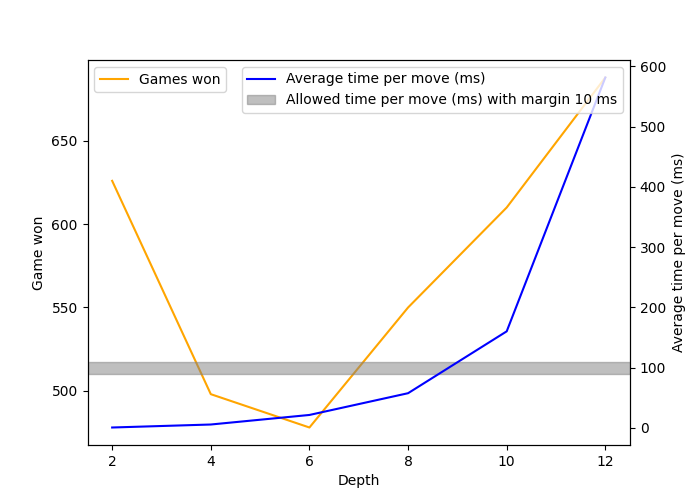
\includegraphics[width=0.8\textwidth]{../img/minimax_config_openworld.png}
  \caption{Comparison of number of wins of different fixed depths parameters in Minimax agent along with average time taken per ply in the open world}
  \label{minimaxOWDepth}
\end{figure}

\subsection{Configuring Minimax Parameters}

In order to optimize the performance of the Minimax agent in an open world environment, we must determine the optimal values for the \texttt{depth} and \texttt{eval} parameters. We will use the playout heuristic for the \texttt{eval} parameter as it is generally superior to the basic heuristic. To find the best value for the \texttt{depth} parameter, I ran a 1000 game experiment that tries different values for it against the Greedy agent. 

Figure \ref{minimaxOWDepth} illustrates the number of games won and the average time taken per ply by the Minimax agent with different depth parameters. The plot shows that the number of games won by the Minimax agent improves as the depth of the game tree exploration increases. The same trend can be observed for the average time taken to make a move. However, it is surprising to see that lower depth values such as 2 and 3 have a higher number of games won than the highest depth value of 6, which has the lowest number of wins. This observation warrants further investigation. Besides this, a horizontal shaded line is included in the plot to represent the optimal average time that the agent should take to make a move. It can be observed that the grey shaded line intersects with the average time of the Minimax agent at a depth of 9. This suggests that, in an open environment, this value of the parameter is the most suitable and will be used in the tournament.

Figure \ref{minimaxOWEval} illustrates the comparison between two heuristic evaluation functions, namely \texttt{basic} and \texttt{playout}, for the Minimax agent with a fixed depth of 9. The left subplot shows the number of games won for the two evaluation functions, and the right subplot displays the average time (ms) taken to make a move. It can be observed that the playout heuristic outperforms the basic heuristic in terms of number of games won, achieving almost twice the number of wins of the basic heuristic. However, the playout heuristic is slower than the basic heuristic, as shown by the right subplot. Despite this, the playout heuristic still performs around the optimal time range of 100ms, making it the preferred choice for the tournament. As a result, the Minimax agent will use the depth 9 and playout heuristic for the tournament.

\begin{figure}[h]
  \centering
  \captionsetup{justification=centering}
  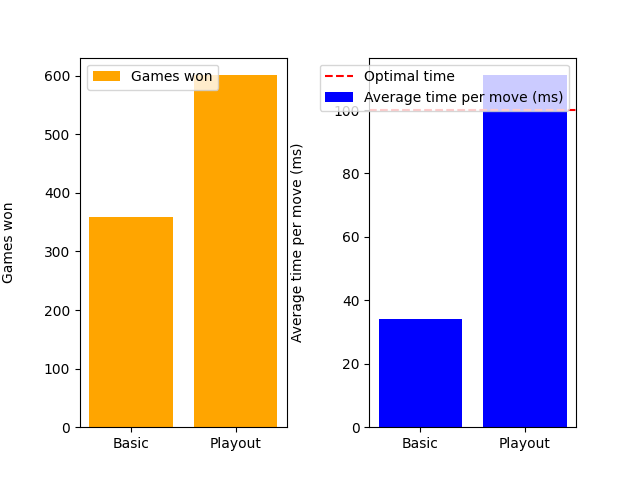
\includegraphics[width=0.8\textwidth]{../img/minimax_eval_openworld.png}
  \caption{Comparison of number of wins and average time taken per ply of \texttt{basic} and \texttt{playout} evaluation functions in Minimax agent in the open world}
  \label{minimaxOWEval}
\end{figure}

\subsection{Configuring MCTS Parameters}

In order to compare MCTS agents with other agents in the open world, it is necessary to determine the optimal values for the parameters \texttt{limit}, \texttt{c}, and \texttt{simulation}. To begin, the exploration constant was set to 1.41, which is typically an optimal value \citep{AI4Ed}, and the \texttt{simulation} was set to \texttt{greedy}. With these parameters in place, an experiment was conducted using 1000 games to find the value of \texttt{limit} by trying various values of iterations to identify the optimal value. The results of this experiment are depicted in Figure \ref{mctsOWIterations}.

\begin{figure}[h!]
  \centering
  \captionsetup{justification=centering}
  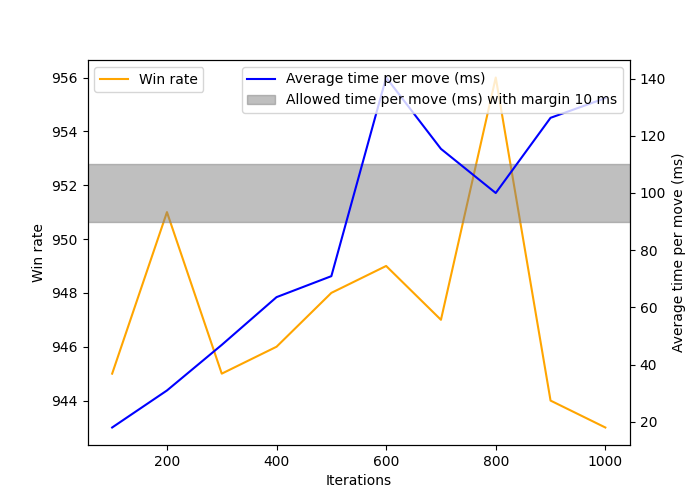
\includegraphics[width=0.8\textwidth]{../img/mcts_iterations_openworld.png}
  \caption{Comparison of win rates and average time taken per ply of different fixed iterations in MCTS algorithm in the open world}
  \label{mctsOWIterations}
\end{figure}

Similar to the Minimax agent, it can be seen that an increase in the number of \texttt{iterations} generally results in a corresponding increase in the average time taken per move, as well as an increase in the win rate. By examining the shaded region in Figure \ref{mctsOWIterations}, which represents the optimal time per move, it can be determined that the optimal value for the \texttt{iterations} parameter is 800. This value results in a relatively high win rate and the lowest average time taken per move.

With the \texttt{iterations} parameter set to 800 and the \texttt{simulation} value remaining at greedy, a new experiment was conducted to determine the optimal value for the \texttt{c} exploration parameter in MCTS. The results of this experiment are shown in Figure \ref{mctsOWC}. From the figure, it can be observed that the optimal value for the \texttt{c} parameter is 1.00, as it yields the highest number of wins while still operating within the optimal average time per move.

\begin{figure}[h!]
  \centering
  \captionsetup{justification=centering}
  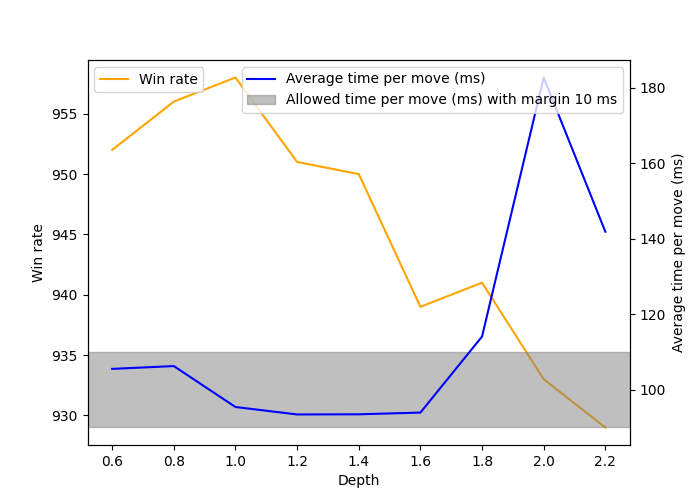
\includegraphics[width=0.8\textwidth]{../img/mcts_c_openworld.png}
  \caption{Comparison of number of wins and average time taken per ply of different fixed exploration parameters in MCTS algorithm in the open world}
  \label{mctsOWC}
\end{figure}

Like in the comparison of heuristic evaluation functions for the Minimax agent, bar plots were used to visualize the number of games won and average times per move for different simulation types in the MCTS algorithm. The left subplot in Figure \ref{mctsOWSimulations} compares the number of games won of the two simulations, and it can be seen that the greedy simulation performs significantly better than the random playouts. Additionally, the greedy simulation is much faster than the random playouts, as can be seen in the right subplot. This is due to the nature of random simulation, as discussed in Section \ref{MCTS}. Based on these results, we can conclude that the optimal parameters for the simulation in MCTS are greedy.

\begin{figure}[h]
  \centering
  \captionsetup{justification=centering}
  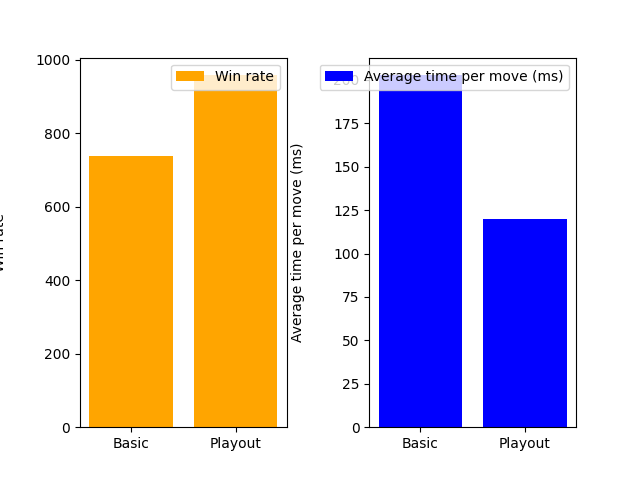
\includegraphics[width=0.8\textwidth]{../img/mcts_simulation_openworld.png}
  \caption{Comparison of number of games won and average time taken per ply of \texttt{random} and \texttt{greedy} simulations in MCTS algorithm in the open world}
  \label{mctsOWSimulations}
\end{figure}

\subsection{Tournament}
In order to begin the tournament, the following list of agents and their corresponding parameters were used: Random, Greedy, Smart, Minimax (depth 9 and playout heuristic evaluation function), and MCTS (limit 800, exploration parameter 1.00 and greedy simulation type).

Furthermore, the game environment was configured with the following settings: open world, including trumps, 500 games and starting rank 6.

The tournament was initiated using the following command, with the aforementioned configurations.

\begin{lstlisting}
$ dotnet run -tournament="random/greedy/smart/minimax:depth=9,eval=playout/mcts:limit=800,c=1.00,simulation=greedy" -total_games=500 -open_world
\end{lstlisting}

It is important to note that \texttt{-include\_trumps} and \texttt{=start\_rank=6} game environment parameters are not explicitly listed in the above command as they are already set to their default values in the game setup.

To improve the readability of the table of tournament results, we will use shortened versions of the long agent names as aliases. The full names and their corresponding aliases are listed below:

\begin{itemize}
	\item \textbf{minimax} := minimax:depth=9:eval=playout
	\item \textbf{mcts} := mcts:limit=800:c=1.00:simulation=greedy
\end{itemize}

\begin{table}[]
\captionsetup{justification=centering}
\begin{tabularx}{\textwidth}{|X|X|X|X|X|X|}
\toprule

                                        & random               & greedy               & smart                & minimax & mcts \\ \midrule
random                                  &                      & \footnotesize{5.6\%-11.3\% (500)}   & \footnotesize{3.3\%-8.0\% (500)}    & \footnotesize{1.2\%-4.6\% (500)}            & \footnotesize{0.0\%-1.1\% (500)}                       \\ \midrule
greedy                                  & \footnotesize{88.7\%-94.4\% (500)}  &                      & \footnotesize{45.7\%-49.9\% (3500)} & \footnotesize{33.5\%-43.6\% (500)}          & \footnotesize{1.1\%-4.4\% (500)}                       \\ \midrule
smart                                   & \footnotesize{92.0\%-96.7\% (500)}  & \footnotesize{50.1\%-54.3\% (3500)} &                      & \footnotesize{34.7\%-45.0\% (500)}          & \footnotesize{2.8\%-7.2\% (500)}                       \\ \midrule
minimax            & \footnotesize{95.4\%-98.8\% (500)}  & \footnotesize{56.4\%-66.5\% (500)}  & \footnotesize{55.0\%-65.3\% (500)}  &                              & \footnotesize{16.4\%-24.8\% (500)}                     \\ \midrule
mcts & \footnotesize{98.9\%-100.0\% (500)} & \footnotesize{95.6\%-98.9\% (500)}  & \footnotesize{92.8\%-97.2\% (500)}  & \footnotesize{75.2\%-83.6\% (500)}          &                                         \\ \bottomrule
\end{tabularx}
    \caption{Tournament between the agents in the open world}
    \label{tournamentOpenWorld}
\end{table}

It should be noted that in this tournament, every pair of agents mentioned in the command line played against each other to determine the winner. These agents did not play against themselves, as this would provide almost the same win rate and the tournament would continue to increase the number of games played for them.

From the Table \ref{tournamentOpenWorld}, the results of the tournament indicate that the MCTS agent with the parameter configuration of \texttt{simulation=greedy}, \texttt{limit=800} and \texttt{c=1.00}  was the clear winner, with a consistently high win rate against all other opponents. In particular, the MCTS agent outperformed the other agents, with win rates of 98.9\%-100.0\% against Random, 95.6\%-98.9\% against Greedy, and 92.8\%-97.2\% against Smart. Due to the dominance of the MCTS algorithm, all results were gathered after 500 games, with no need for additional increments.

The Minimax agent performed performed well against the Random, Greedy and Smart agents, although its results were not as strong as those of the MCTS agent. However, 500 games were sufficient to identify the clear winner in these matchups. 

In summary, the MCTS agent with the specified parameter configuration emerged as the clear winner in terms of win rate, with a strong performance against all other agents. The Minimax agent with the specified parameter configuration came in second, with strong performances against the random, greedy, and smart agents. The smart agent came in third, with a win rate that outperformed the greedy agent, although it took 3500 simulations to find a significant winner between the two. The greedy agent came in fourth, while the random agent had the lowest win rate among all agents. Overall, these results indicate that the MCTS and Minimax agents with their respective parameter configurations are the most effective at winning games, while also having good performance in terms of average time per move.

\section{Closed world}

While the open world setting provides a useful reference point for evaluating the performance of different agents, it is also important to consider how they perform in a closed world environment. As previously mentioned, the normal game of Durak is played in a closed world, with players only able to see their own cards and the trump card that is face up. In this section, we will examine the performance of various agents in a closed world setting and compare it to their performance in the open world. Similar to the open world setting, it is necessary to configure the parameters for Minimax and MCTS agents in a closed world environment in order to optimize their performance. This configuration process includes setting the value of the additional \texttt{samples} parameter to find the frequent move in the hidden state (details in Section \ref{closedWorld}. To determine the optimal values for all relevant parameters, a series of games will be conducted to identify the values that are most suitable for the tournament environment just like before. It is important to ensure that the selected parameters result in an average move time of around 100ms in order to identify the most efficient configuration for the agent.

\subsection{Configuring Minimax Parameters}

In order to optimize the performance of the Minimax agent in an closed world environment, we must determine the optimal values for the \texttt{depth}, \texttt{eval} and \texttt{samples} parameters. We will use the playout heuristic for the \texttt{eval} parameter as it is generally superior to the basic heuristic and set the value 10 to the \texttt{samples} parameter, as this value allows for a faster search process while still providing sufficient information to identify the most frequent move. To find the best value for the \texttt{depth} parameter, I ran a 100 game experiment that tries different values for it against the Greedy agent. The decrease in the number of games can be attributed to the fact that searching for optimal moves using strategies like Minimax and MCTS becomes slower in a closed world environment. This is because these strategies require sampling the game state a specific number of times, the value of \texttt{samples}, in order to determine the most frequent move, which can be time-consuming.

\begin{figure}[h]
  \centering
  \captionsetup{justification=centering}
  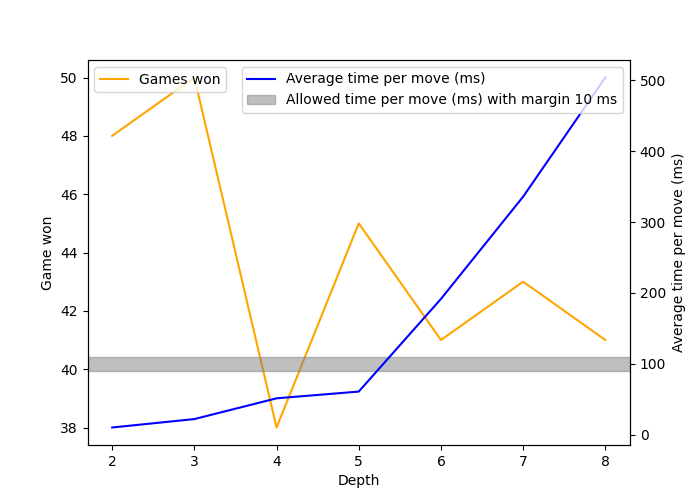
\includegraphics[width=0.8\textwidth]{../img/minimax_depth_closedworld.png}
  \caption{Comparison of number of games won of different fixed depths parameters in Minimax agent along with average time taken per ply in the closed world}
  \label{minimaxCWDepth}
\end{figure}

Figure \ref{minimaxCWDepth} illustrates the number of games won and the average time taken per ply by the Minimax agent with different depth parameters in the closed world. Unlike the open world, the plot shows that the number of games won by the Minimax agent does not improve as the depth of the game tree exploration increases. One potential reason for the lack of an increase in the win rate as the depth increases is that the value of the samples is not large enough. This may prevent the search process from considering all possible moves, leading to the selection of suboptimal moves. The average time taken to make a move, on the other hand, does follow the trend just like the open world: takes more time to make a move as the depth increases. It is unexpected to see that the number of games won fluctuates as the value of the depth parameter increases. This phenomenon warrants further investigation to understand the underlying cause. It can be observed that the highest number of games won is achieved when the depth parameter is set to 3. In addition to providing the best results, this setting also results in relatively fast move times. This suggests that, in the closed environment, this value of the parameter is the most suitable and will be used in the tournament.

\begin{figure}[h]
  \centering
  \captionsetup{justification=centering}
  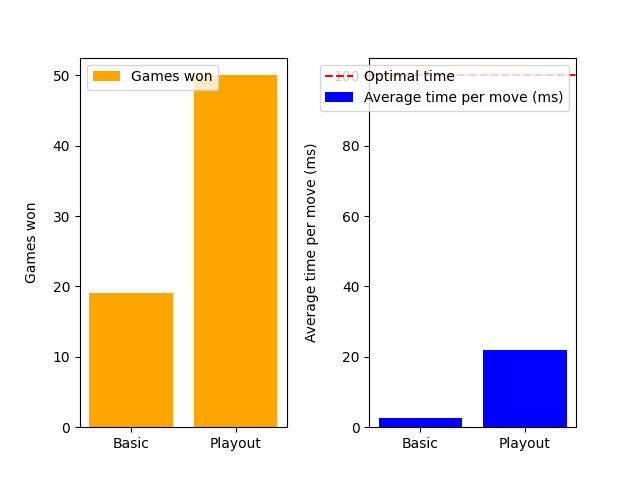
\includegraphics[width=0.8\textwidth]{../img/minimax_eval_closedworld.png}
  \caption{Comparison of number of wins and average time taken per ply of \texttt{basic} and \texttt{playout} evaluation functions in Minimax agent in the closed world}
  \label{minimaxCWEval}
\end{figure}

As shown in Figure \ref{minimaxCWEval}, the performance of two heuristic evaluation functions, namely \texttt{basic} and \texttt{playout}, is compared for a Minimax agent with a fixed \texttt{depth} of 3 and a fixed number of \texttt{samples} of 10 in a closed world environment. The left subplot presents the number of games won for the two evaluation functions, while the right subplot displays the average time taken to make a move. It can be observed that, similar to the open world setting, the playout heuristic outperforms the basic heuristic in terms of the number of games won, achieving more than twice as many wins as the basic heuristic. However, the playout heuristic is slower than the basic heuristic, as indicated by the right subplot. Despite this, the playout heuristic still performs within the optimal time range of 100ms, making it the preferred choice for the tournament. As a result, the Minimax agent will use the depth 9 and playout heuristic for the tournament.

In contrast to the open world setting, it is necessary to identify an appropriate value for the \texttt{samples} parameter in addition to the already-configured parameters in a closed world environment. Figure \ref{minimaxCWSamples} illustrates the experiment that was conducted to determine the optimal value for the \texttt{samples} parameter for the tournament. It indicates that the optimal value for the \texttt{samples} parameter is 30, as it results in the highest number of games won compared to the other tested values. This information can be used to determine the final parameter configuration for the Minimax agent. As a result, the Minimax agent will use the depth 3, playout heuristic and the samples 30 for the tournament.

\begin{figure}[h]
  \centering
  \captionsetup{justification=centering}
  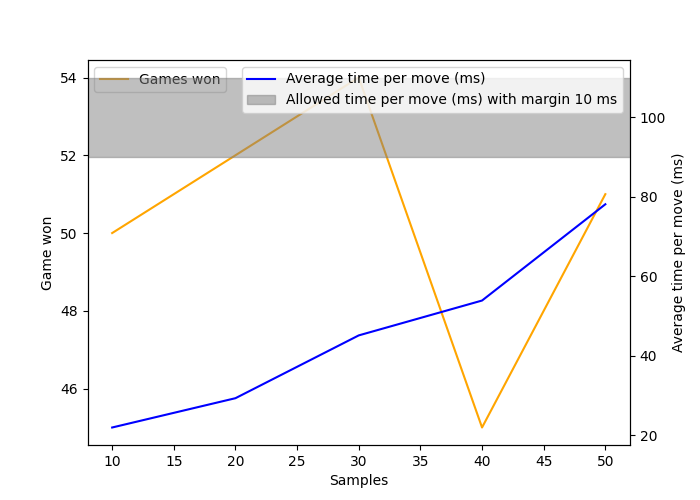
\includegraphics[width=0.8\textwidth]{../img/minimax_samples_closedworld.png}
  \caption{Comparison of number of wins and average time taken per ply of the \texttt{samples} value in Minimax agent in the closed world}
  \label{minimaxCWSamples}
\end{figure}




\subsection{Configuring MCTS Parameters}

To compare MCTS agents with other agents in an closed world environment tournament, it is necessary to determine the optimal values for the \texttt{limit}, \texttt{c}, \texttt{simulation} and \texttt{samples} parameters. As a starting point, the exploration constant was set to 1.41, which is generally considered an optimal value based on previous research \citep{AI4Ed}, the simulation parameter was set to \texttt{greedy} and the samples parameter was set to 10. With these parameters in place, an experiment involving 100 games was conducted to identify the optimal value for the limit parameter by testing various values for the number of iterations. The results of this experiment are shown in Figure \ref{mctsCWIterations}.

\begin{figure}[h]
  \centering
  \captionsetup{justification=centering}
  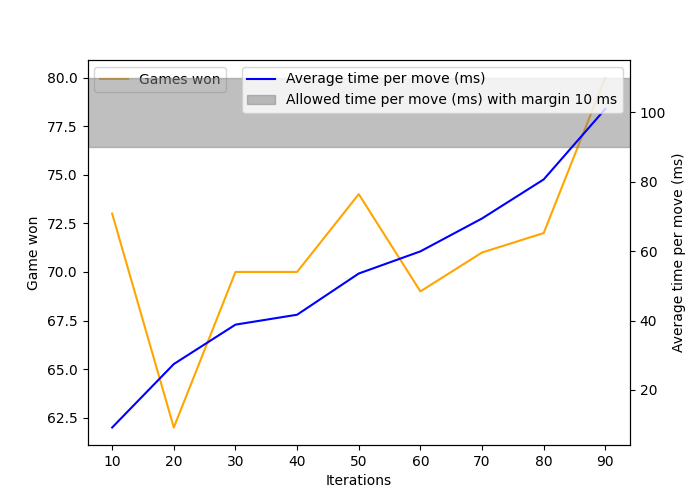
\includegraphics[width=0.8\textwidth]{../img/mcts_iterations_closedworld.png}
  \caption{Comparison of win rates and average time taken per ply of different fixed iterations in MCTS algorithm in the closed world}
  \label{mctsCWIterations}
\end{figure}

Similar to the Minimax agent, it can be seen that an increase in the number of \texttt{iterations} generally results in a corresponding increase in the average time taken per move, as well as an increase in the win rate. However, it is not clear why the number of games won using the value 10 for the iterations parameter is higher than the result of value of 20. This observation warrants further investigation in order to understand the underlying cause. By examining the shaded region in Figure \ref{mctsCWIterations}, which represents the optimal time per move, it can be determined that the optimal value for the \texttt{iterations} parameter is 90 in the closed world. This value results in a relatively high win rate and the lowest average time taken per move.

With the \texttt{iterations} parameter set to 90, the \texttt{simulation} value remaining at greedy and \texttt{samples} value remaining at 10, a new experiment was conducted to determine the optimal value for the \texttt{c}, exploration parameter, in MCTS. The results of this experiment are shown in Figure \ref{mctsCWC}. From the figure, it can be observed that the optimal value for the \texttt{c} parameter is 1.40, as it yields the highest number of wins while still operating within the optimal average time per move.

\begin{figure}[h]
  \centering
  \captionsetup{justification=centering}
  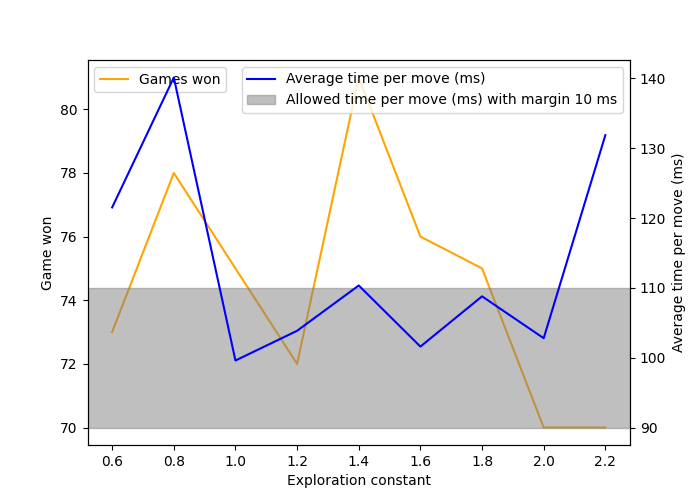
\includegraphics[width=0.8\textwidth]{../img/mcts_c_closedworld.png}
  \caption{Comparison of number of wins and average time taken per ply of different fixed exploration parameters in MCTS algorithm in the closed world}
  \label{mctsCWC}
\end{figure}

Like in the comparison of heuristic evaluation functions for the Minimax agent, bar plots were used to visualize the number of games won and average times per move for different simulation types in the MCTS algorithm. The left subplot in Figure \ref{mctsCWSimulations} compares the number of games won of the two simulations, and it can be seen that the greedy simulation performs significantly better than the random playouts. Additionally, the greedy simulation is much faster than the random playouts, as can be seen in the right subplot. This is due to the nature of random simulation, as discussed in Section \ref{MCTS}. Based on these results, we can conclude that the optimal parameters for the simulation in MCTS are greedy.

\begin{figure}[h!]
  \centering
  \captionsetup{justification=centering}
  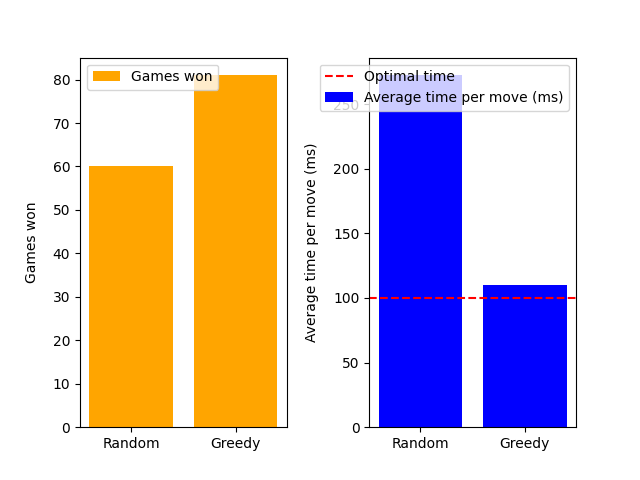
\includegraphics[width=0.8\textwidth]{../img/mcts_simulation_closedworld.png}
  \caption{Comparison of number of games won and average time taken per ply of \texttt{random} and \texttt{greedy} simulations in MCTS algorithm in the closed world}
  \label{mctsCWSimulations}
\end{figure}

The results of the experiment conducted to determine the optimal value of the \texttt{samples} parameter for the MCTS agent in the closed-world tournament are shown in Figure \ref{mctsCWSamples}. In this experiment, the optimal value for the samples parameter will be determined by treating the limit parameter as a \textbf{total budget}. Given a total budget of 900, the number of iterations can be calculated by dividing the budget by the value of the samples parameter. For example, if the samples parameter is set to 10, there will be 900/10 = 90 iterations in each sample game. Previous analysis has shown that the optimal value for the limit parameter is 90 when the samples parameter is set to 10. Therefore, a total budget of 900 will be used in this experiment to determine the optimal value for the samples parameter.

It can be seen that the highest number of games won is achieved with a samples value of 30, which corresponds to the limit value of 900 / 30 = 30. Based on these results, the MCTS agent will be configured with a limit of 30, an exploration constant of 1.40, a greedy simulation type, and a samples value of 30 for the closed-world tournament.

\begin{figure}[h]
  \centering
  \captionsetup{justification=centering}
  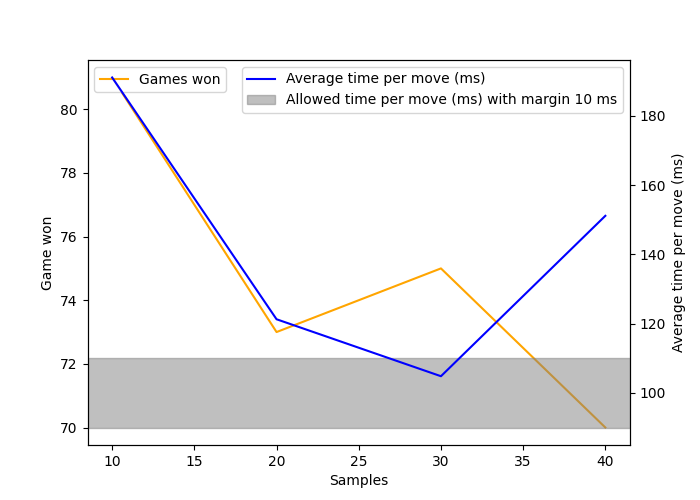
\includegraphics[width=0.8\textwidth]{../img/mcts_samples_closedworld.png}
  \caption{Comparison of number of wins and average time taken per ply of the \texttt{samples} value in MCTS agent in the closed world}
  \label{mctsCWSamples}
\end{figure}

\begin{table}[!ht]
    \centering
    \captionsetup{justification=centering}
    \begin{tabularx}{\textwidth}{|X|X|X|X|X|X|}
    \hline
        ~ & random & greedy & smart & minimax & mcts \\ \hline
        random & ~ & \footnotesize{5.6\%-11.3\% (500)} & \footnotesize{3.8\%-8.7\% (500)} & \footnotesize{4.3\%-9.5\% (500)} & \footnotesize{0.4\%-2.7\% (500)} \\ \hline
        greedy & \footnotesize{88.7\%-94.4\% (500)} & ~ & \footnotesize{49.4\%-51.9\% (10000)} & \footnotesize{45.7\%-49.2\% (4500)} & \footnotesize{14.9\%-23.2\% (500)} \\ \hline
        smart & \footnotesize{91.3\%-96.2\% (500)} & \footnotesize{48.1\%-50.6\% (10000)} & ~ & \footnotesize{50.1\%-57.5\% (1000)} & \footnotesize{22.2\%-31.6\% (500)} \\ \hline
        minimax & \footnotesize{90.5\%-95.7\% (500)} & \footnotesize{50.8\%-54.3\% (4500)} & \footnotesize{42.5\%-49.9\% (1000)} & ~ & \footnotesize{12.9\%-20.6\% (500)} \\ \hline
        mcts & \footnotesize{97.3\%-99.6\% (500)} & \footnotesize{76.8\%-85.1\% (500)} & \footnotesize{68.4\%-77.8\% (500)} & \footnotesize{78.4\%-87.3\% (500)} & \\ \bottomrule
    \end{tabularx}
    \caption{Tournament between the agents in the closed world}
    \label{tournamentClosedWorld}
\end{table}

\subsection{Tournament}
In order to begin the tournament, the following list of agents and their corresponding parameters were used: Random, Greedy, Smart, Minimax (depth 3, playout heuristic evaluation function and samples 30), and MCTS (limit 30, exploration parameter 1.40, greedy simulation type and samples value 30).

Furthermore, the game environment was configured with the following settings: closed world, including trumps, 500 games and starting rank 6.

The tournament was initiated using the following command, with the aforementioned configurations.

\begin{lstlisting}
$ dotnet run -tournament="random/greedy/smart/minimax:depth=3,eval=playout,samples=30/mcts:limit=30,c=1.40,simulation=greedy,samples=30" -total_games=500
\end{lstlisting}

To improve the readability of the table of tournament results, we will use shortened versions of the long agent names as aliases. The full names and their corresponding aliases are listed below:

\begin{itemize}
	\item \textbf{minimax} := minimax:depth=3:eval=playout,samples=30
	\item \textbf{mcts} := mcts:limit=30:c=1.40:simulation=greedy,samples=30
\end{itemize}


It should be noted that in this tournament, every pair of agents mentioned in the command line played against each other to determine the winner. These agents did not play against themselves, as this would provide almost the same win rate and the tournament would continue to increase the number of games played for them.

In addition to the open world environment results, the MCTS agent with the parameter configuration of \texttt{simulation=greedy}, \texttt{limit=30}, \texttt{c=1.40}, and \texttt{samples=30} also demonstrated dominance in the closed world environment. From the Table \ref{tournamentClosedWorld}, the results of the tournament indicate that the MCTS agent outperformed the other agents, with win rates of 97.3\%-99.6\% against Random, 76.8\%-85.1\% against Greedy, 68.4\%-77.8\% against Smart and 79.4\%-87.1\% against Minimax. Due to the dominance of the MCTS algorithm, all results were gathered after 500 games, with no need for additional increments. These results indicate that this MCTS agent is the clear winner in both perfect and imperfect information settings in the game of Durak. Overall, the MCTS algorithm performs exceptionally well in this game, consistently achieving high win rates against other agents.

In the closed world scenario, the minimax agent performed less well compared to its performance in the open world. This suggests that the agent's performance varies depending on the type of environment it is in. In the open world, the minimax agent achieved a high win rate against all other agents except the MCTS agent; MCTS won. However, in the closed world, the minimax agent also lost to the Smart agent. This may be due to the fact that the limit on average time per move does not allow the the current configuration of the minimax parameters to explore the game tree reasonable to make a better move, leading to its decreased performance against the Smart agent.

Table \ref{tournamentClosedWorld} shows that the performance of the Greedy and Smart agents is comparable in the closed world environment. The number of games played to determine a clear winner reached the upper bound of 10,000 games. In contrast to the open world, the Smart agent appears to be weaker in the closed world. This  due to the fact that the Smart agent relies on knowledge of the opponent's hand to inform its strategies, which is not available in the closed world setting. As a result, the Smart agent's performance is affected in this environment.

In summary, the results of the closed world tournament show that the MCTS agent with the specified parameter configuration had the highest win rate among all agents, with strong performance against all other competitors. The Smart agent was the second most successful, achieving good results against the Random and Minimax agents. However, the Smart agent's performance was comparable to that of the Greedy agent. The Minimax agent with the specified parameter configuration ranked third in terms of win rate, followed by the Greedy agent, while the Random agent had the lowest win rate. Overall, these results suggest that the MCTS agent and the Smart agent are the most effective at winning closed-world games, and also have good performance in terms of average time per move.

\section{The Advantage of the First Moving Player}

Initially, it is determined that the player with the lowest trump card will make the first move. If neither player holds a trump card, the first player is randomly chosen (details in Section \ref{dealingCards}). In order to determine if the first player has an advantage, an experiment was conducted in which two random, two greedy, two minimax, and two MCTS agents played against each other. Each of the experiments had 100 games in the open world environment. The parameters for Minimax, \texttt{depth=4} and \texttt{eval=playout}, and MCTS, \texttt{limit=50}, \texttt{c=1.41} and \texttt{simulation=greedy}, were set arbitrarily (details regarding their parameters in Section \ref{paramSpecification}). The results are depicted in Figure \ref{firstmoveadvantage}.

\begin{figure}[h]
  \centering
  \captionsetup{justification=centering}
  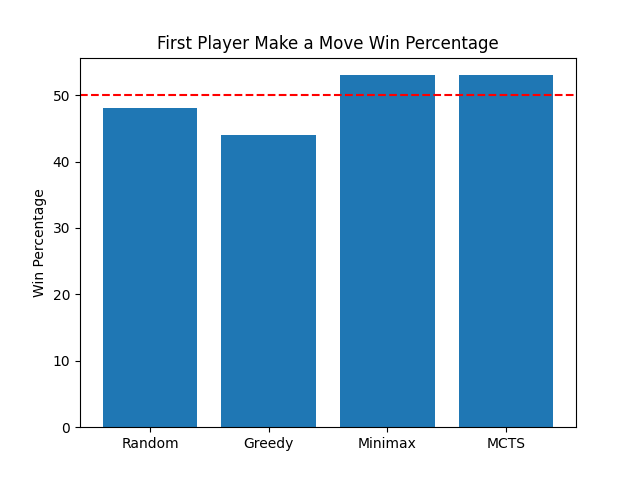
\includegraphics[width=0.8\textwidth]{../img/advantage.png}
  \caption{First player making a move win percentage with Random, Greedy, Minimax, and MCTS}
  \label{firstmoveadvantage}
\end{figure}

The results of the experiment, depicted in Figure \ref{firstmoveadvantage}, indicate that making the first move does not have a significant advantage for basic strategies such as random and greedy. Specifically, the random agents won 48 out of 100 games when making the first move, and the greedy agents won 44 out of 100 games under the same circumstances. On the other hand, more complex strategies such as minimax and MCTS appear to benefit from making the first move, with the minimax agents winning 53 out of 100 games and the MCTS agents also winning 53 out of 100 games. While the results suggest that the first player has a slight advantage when using more advanced strategies and does not have a slight advantage when using the basic strategies, the difference in win rate is not extreme, with the win rate for all strategies hovering around 50\%. Therefore, it can be concluded that making the first move does not have a significant impact on the outcome of the game.

\chapter*{Conclusion}
\addcontentsline{toc}{chapter}{Conclusion}

In conclusion, this thesis provided a detailed description and analysis of the card game Durak, as well as the development of a game and AI framework for implementing and testing different agents. Through the implementation and experimentation of various agents, including Minimax, Rule-Based, and MCTS, the MCTS agent consistently outperformed the other agents in both perfect and imperfect information versions of Durak.

The results of this study demonstrate the effectiveness of the MCTS approach for developing AI agents that can perform well in the Durak game. The various parameters used in the MCTS agent, such as the \texttt{iterations}, \texttt{exploration constant} and the \texttt{simulation} strategy, played a crucial role in determining its performance. By carefully tuning these parameters, it was possible to achieve strong results across a range of experimental conditions in both perfect and imperfect information scenarios.

\chapter*{Future Work}

Future work on this project could involve the implementation of additional agents beyond Minimax and MCTS. Some possibilities could include evolutionary algorithms, reinforcement learning, or other search-based approaches.

Another direction for future work could be to extend the game to other variations of Durak, such as Durak with fooling or Durak with transfers or even Passports. These variations introduce additional rules and complexity to the game, which could provide interesting challenges for the agents to tackle.

In the experiments, it would be interesting to run a tournament between the agents with the trump cards removed. This would provide valuable insight into the influence of the trump cards on the agents' performance and whether the same agent can perform well in this modified environment.

Another area for future work could be to improve the rule-based agents in this framework. One possibility could be to expand the set of rules that the agent uses besides the weaknesses to make decisions, potentially incorporating more advanced strategies and tactics. Additionally, it might be useful to explore ways of incorporating additional information, such as the cards that have already been played, into the rule-based agent's decision-making process to improve its performance.

Also, improving the heuristic function of the Minimax agent could be a useful direction for future work. The current implementation of the heuristic function relies on a relatively small number of criteria to evaluate the state of the game, such as the number of cards in the player's hand, the value of the hand and the existence of weaknesses.

Another direction for future work could be to improve the optimization technique of state caching in the current implementation of the Minimax agent. While the current implementation does include this feature, the results of experiments comparing the use of state caching versus not using it have shown relatively little difference in performance.

%%% Bibliography
%%% Bibliography (literature used as a source)
%%%
%%% We employ bibTeX to construct the bibliography. It processes
%%% citations in the text (e.g., the \cite{...} macro) and looks up
%%% relevant entries in the bibliography.bib file.
%%%
%%% The \bibliographystyle command selects, which style will be used
%%% for references from the text. The argument in curly brackets is
%%% the name of the corresponding style file (*.bst). Both styles
%%% mentioned in this template are included in LaTeX distributions.

\bibliographystyle{plainnat}    %% Author (year)
% \bibliographystyle{unsrt}     %% [number]

\renewcommand{\bibname}{Bibliography}

%%% Generate the bibliography. Beware that if you cited no works,
%%% the empty list will be omitted completely.

\bibliography{bibliography}

%%% If case you prefer to write the bibliography manually (without bibTeX),
%%% you can use the following. Please follow the ISO 690 standard and
%%% citation conventions of your field of research.

% \begin{thebibliography}{99}
%
% \bibitem{lamport94}
%   {\sc Lamport,} Leslie.
%   \emph{\LaTeX: A Document Preparation System}.
%   2nd edition.
%   Massachusetts: Addison Wesley, 1994.
%   ISBN 0-201-52983-1.
%
% \end{thebibliography}


%%% Figures used in the thesis (consider if this is needed)
\listoffigures

%%% Tables used in the thesis (consider if this is needed)
%%% In mathematical theses, it could be better to move the list of tables to the beginning of the thesis.
\listoftables

%%% Abbreviations used in the thesis, if any, including their explanation
%%% In mathematical theses, it could be better to move the list of abbreviations to the beginning of the thesis.
\chapwithtoc{List of Abbreviations}

%%% Attachments to the bachelor thesis, if any. Each attachment must be
%%% referred to at least once from the text of the thesis. Attachments
%%% are numbered.
%%%
%%% The printed version should preferably contain attachments, which can be
%%% read (additional tables and charts, supplementary text, examples of
%%% program output, etc.). The electronic version is more suited for attachments
%%% which will likely be used in an electronic form rather than read (program
%%% source code, data files, interactive charts, etc.). Electronic attachments
%%% should be uploaded to SIS and optionally also included in the thesis on a~CD/DVD.
%%% Allowed file formats are specified in provision of the rector no. 72/2017.
\appendix
\chapter{Attachments}

\section{First Attachment}

\openright
\end{document}
